% THIS DOCUMENT IS FOLLOWS THE VOLERE TEMPLATE BY Suzanne Robertson and James Robertson
% ONLY THE SECTION HEADINGS ARE PROVIDED
%
% Initial draft from https://github.com/Dieblich/volere
%
% Risks are removed because they are covered by the Hazard Analysis
\documentclass[12pt]{article}

\usepackage{booktabs}
\usepackage{tabularx}
\usepackage{hyperref}
\usepackage{graphicx}
\usepackage{array}
\graphicspath{ {./diagrams/} }
\hypersetup{
    bookmarks=true,         % show bookmarks bar?
      colorlinks=true,      % false: boxed links; true: colored links
    linkcolor=red,          % color of internal links (change box color with linkbordercolor)
    citecolor=green,        % color of links to bibliography
    filecolor=magenta,      % color of file links
    urlcolor=cyan           % color of external links
}

\newcommand{\lips}{\textit{Insert your content here.}}

%% Comments

\usepackage{color}

\newif\ifcomments\commentstrue %displays comments
%\newif\ifcomments\commentsfalse %so that comments do not display

\ifcomments
\newcommand{\authornote}[3]{\textcolor{#1}{[#3 ---#2]}}
\newcommand{\todo}[1]{\textcolor{red}{[TODO: #1]}}
\else
\newcommand{\authornote}[3]{}
\newcommand{\todo}[1]{}
\fi

\newcommand{\wss}[1]{\authornote{blue}{SS}{#1}} 
\newcommand{\plt}[1]{\authornote{magenta}{TPLT}{#1}} %For explanation of the template
\newcommand{\an}[1]{\authornote{cyan}{Author}{#1}}

%% Common Parts

\newcommand{\progname}{Software Engineering} % PUT YOUR PROGRAM NAME HERE
\newcommand{\authname}{Team 8 -- Rhythm Rangers\\
\\ Ansel Chen
\\ Muhammad Jawad
\\ Mohamad-Hassan Bahsoun
\\ Matthew Baleanu
\\ Ahmed Al-Hayali} % AUTHOR NAMES                  

\usepackage{hyperref}
    \hypersetup{colorlinks=true, linkcolor=blue, citecolor=blue, filecolor=blue,
                urlcolor=blue, unicode=false}
    \urlstyle{same}
                                


\begin{document}

\title{Software Requirements Specification for \progname: subtitle describing software} 
\author{\authname}
\date{\today}
	
\maketitle

~\newpage

\pagenumbering{roman}

\tableofcontents

~\newpage

\section*{Revision History}

\begin{tabularx}{\textwidth}{p{3cm}p{2cm}X}
\toprule {\textbf{Date}} & {\textbf{Version}} & {\textbf{Notes}}\\
\midrule
Date 1 & 1.0 & Notes\\
Date 2 & 1.1 & Notes\\
\bottomrule
\end{tabularx}

~\\

~\newpage
\section{Purpose of the Project}
\subsection{User Business}
\lips
\subsection{Goals of the Project}
\lips
\section{Stakeholders}
\subsection{Client}
\lips
\subsection{Customer}
\lips
\subsection{Other Stakeholders}
\lips
\subsection{Hands-On Users of the Project}
\lips
\subsection{Personas}
\lips
\subsection{Priorities Assigned to Users}
\lips
\subsection{User Participation}
\lips
\subsection{Maintenance Users and Service Technicians}
\lips

\section{Mandated Constraints}
\subsection{Solution Constraints}
\lips
\subsection{Implementation Environment of the Current System}
\lips
\subsection{Partner or Collaborative Applications}
\lips
\subsection{Off-the-Shelf Software}
\lips
\subsection{Anticipated Workplace Environment}
\lips
\subsection{Schedule Constraints}
\lips
\subsection{Budget Constraints}
\lips
\subsection{Enterprise Constraints}
\lips

\section{Naming Conventions and Terminology}
\subsection{Glossary of All Terms, Including Acronyms, Used by Stakeholders
involved in the Project}
\lips

\section{Relevant Facts And Assumptions}
\subsection{Relevant Facts}
\lips
\subsection{Business Rules}
\lips
\subsection{Assumptions}
\lips

\section{The Scope of the Work}
\subsection{The Current Situation}
\lips
\subsection{The Context of the Work}
\lips
\subsection{Work Partitioning}
\lips
\subsection{Specifying a Business Use Case (BUC)}
\lips

\section{Business Data Model and Data Dictionary}
\subsection{Business Data Model}
\lips
\subsection{Data Dictionary}
\lips

\section{The Scope of the Product}
\subsection{Product Boundary}
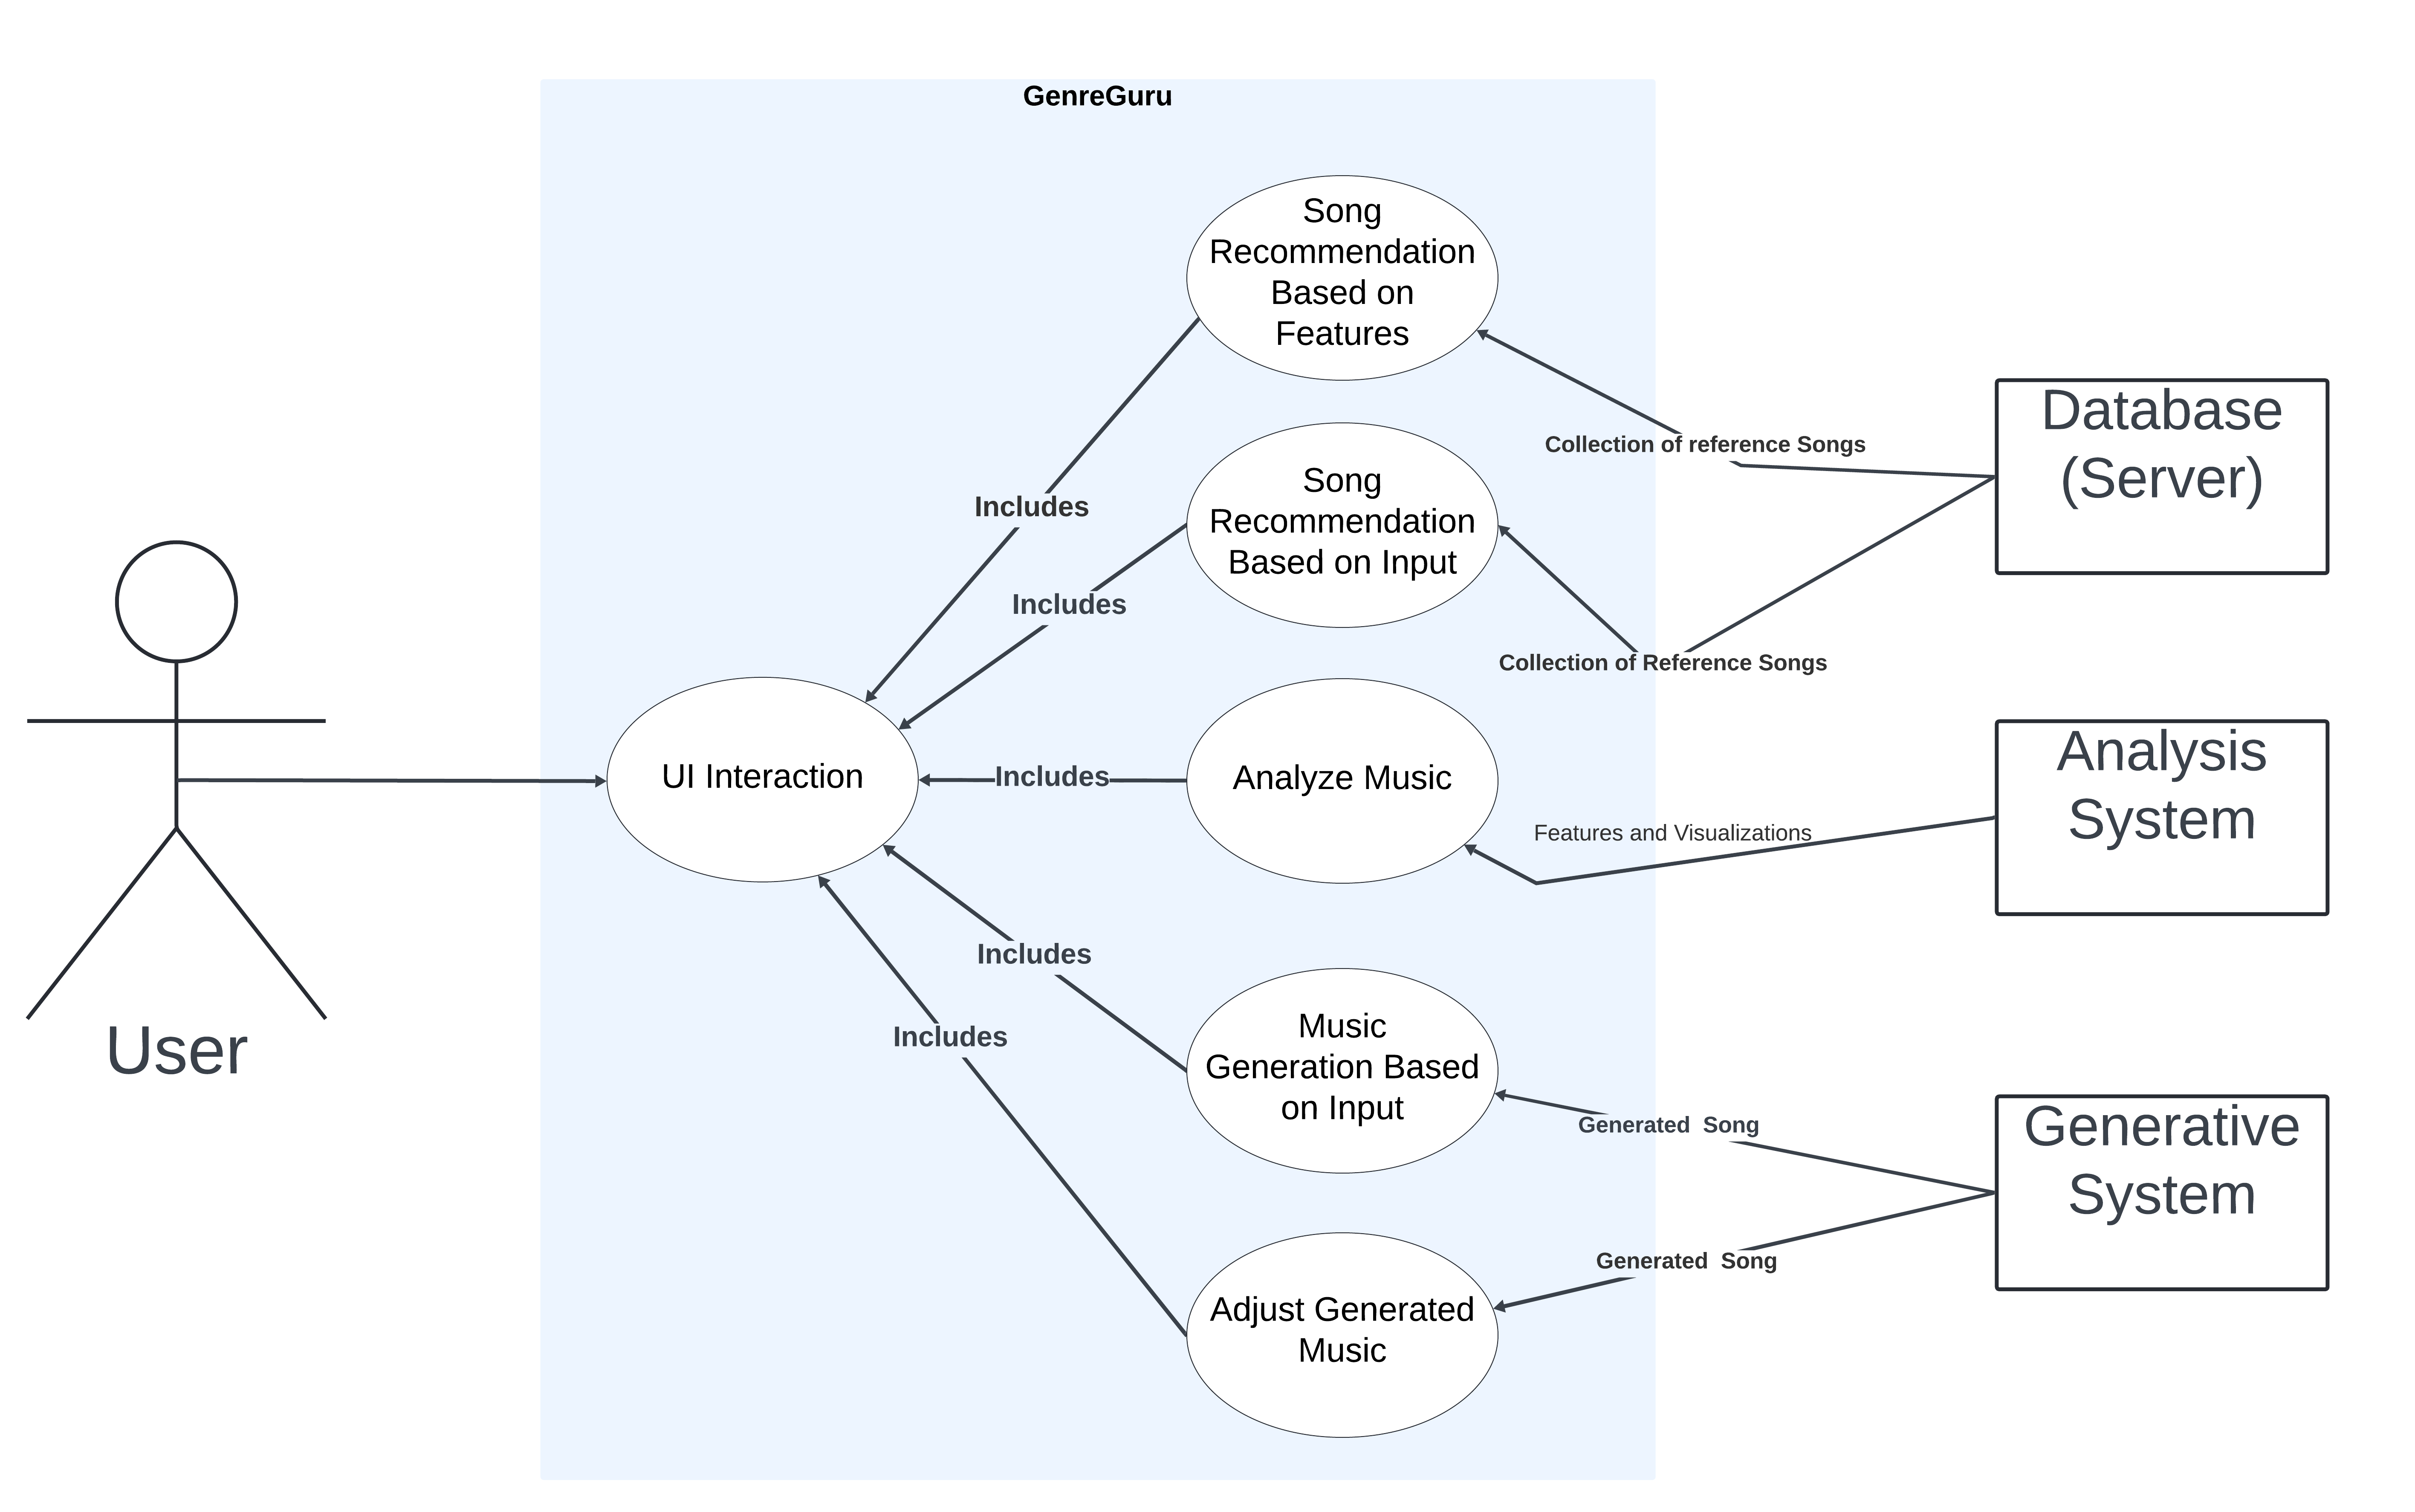
\includegraphics[width=\textwidth]{product_boundary.png} \\
\subsection{Product Use Case Table}
\begin{table}[!ht]
    \centering
    \resizebox{\textwidth}{!}{
    \begin{tabular}{|l|l|l|l|}
    \hline
        \textbf{PUC No} & \textbf{PUC Name} & \textbf{Actor/s} & \textbf{Input \& Output} \\ \hline
        1 & UI Interaction & User & User Actions (click, swipe, drag) (in) \newline System Response (out) \\ \hline
        2 & Song Recommendation Based on Features & User & User's desired features (in) \newline Collection of reference songs (out) \\ \hline
        3 & Music Generation Based on Input & User & Reference song(s) and/or song snippet(s) (in) \newline Generated song or song snippet (out) \\ \hline
        4 & Analyze Music & User & Reference song or song snippet (in) \newline Collection of features and visualizations (out) \\ \hline
        5 & Song Recommendation Based on Input & User & Reference song(s) (in) \newline Collection of reference songs (out) \\ \hline
    \end{tabular}
    }
    \caption{Product Use Case Table}
    \label{tab:PUCtable}
\end{table}

\subsection{Individual Product Use Cases (PUC's)}
\textbf{1. Product Use Case Name:} UI Interaction \\
\textbf{Trigger:} User commits some action (e.g. clicking, swiping, dragging) \\
\textbf{Preconditions:} User has successfully accessed GenreGuru, or is already in GenreGuru \\
\textbf{Interested Stakeholders:} All \\
\textbf{Actor/s:} User \\
\textbf{Activity Diagram:} \\
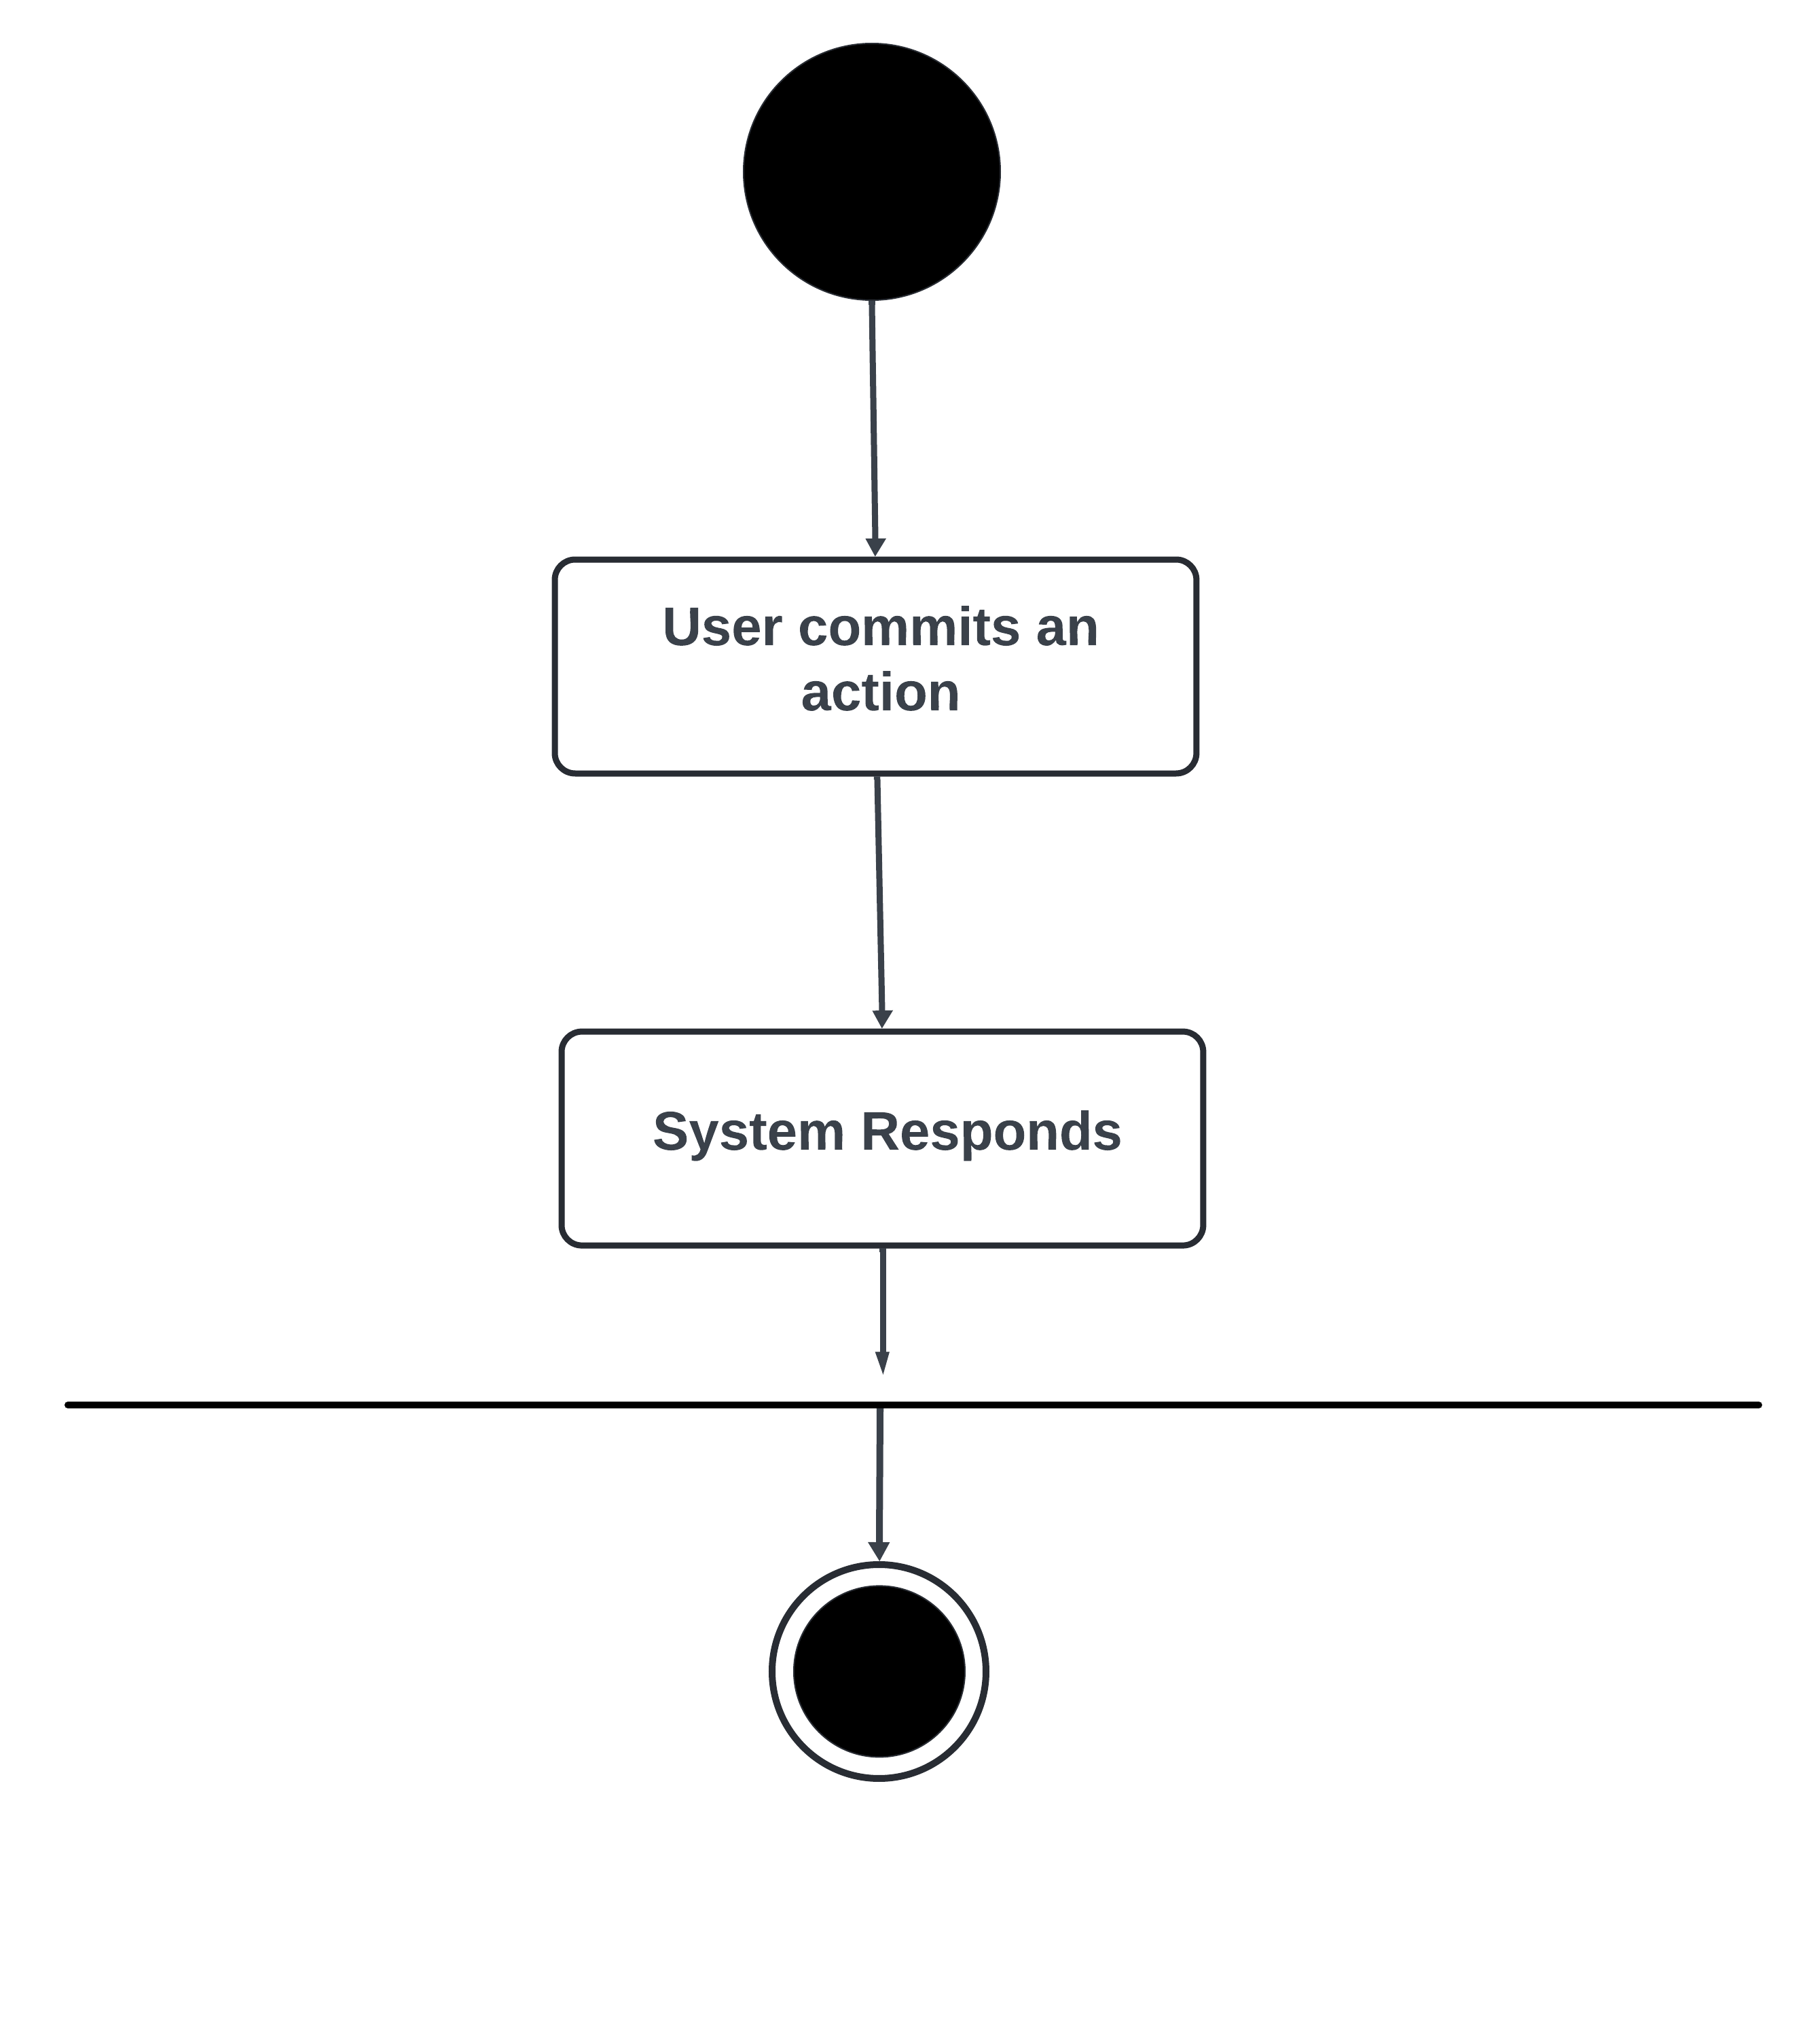
\includegraphics[width=\textwidth]{UI.png} \\
\textbf{Outcome:} The user will commit an action like swiping or pressing and the system will react depending on the action.

\vspace{1cm}

\noindent \textbf{2. Product Use Case Name:} Song Recommendation Based on Features \\
\textbf{Trigger:} User picks features, and indicates they want to search for recommendations \\
\textbf{Preconditions:} User must have GenreGuru open, the user has selected features to search for \\
\textbf{Interested Stakeholders:} Casual Music Listeners, Hobbyist Musicians \\
\textbf{Actor/s:} User \\
\textbf{Activity Diagram:} \\
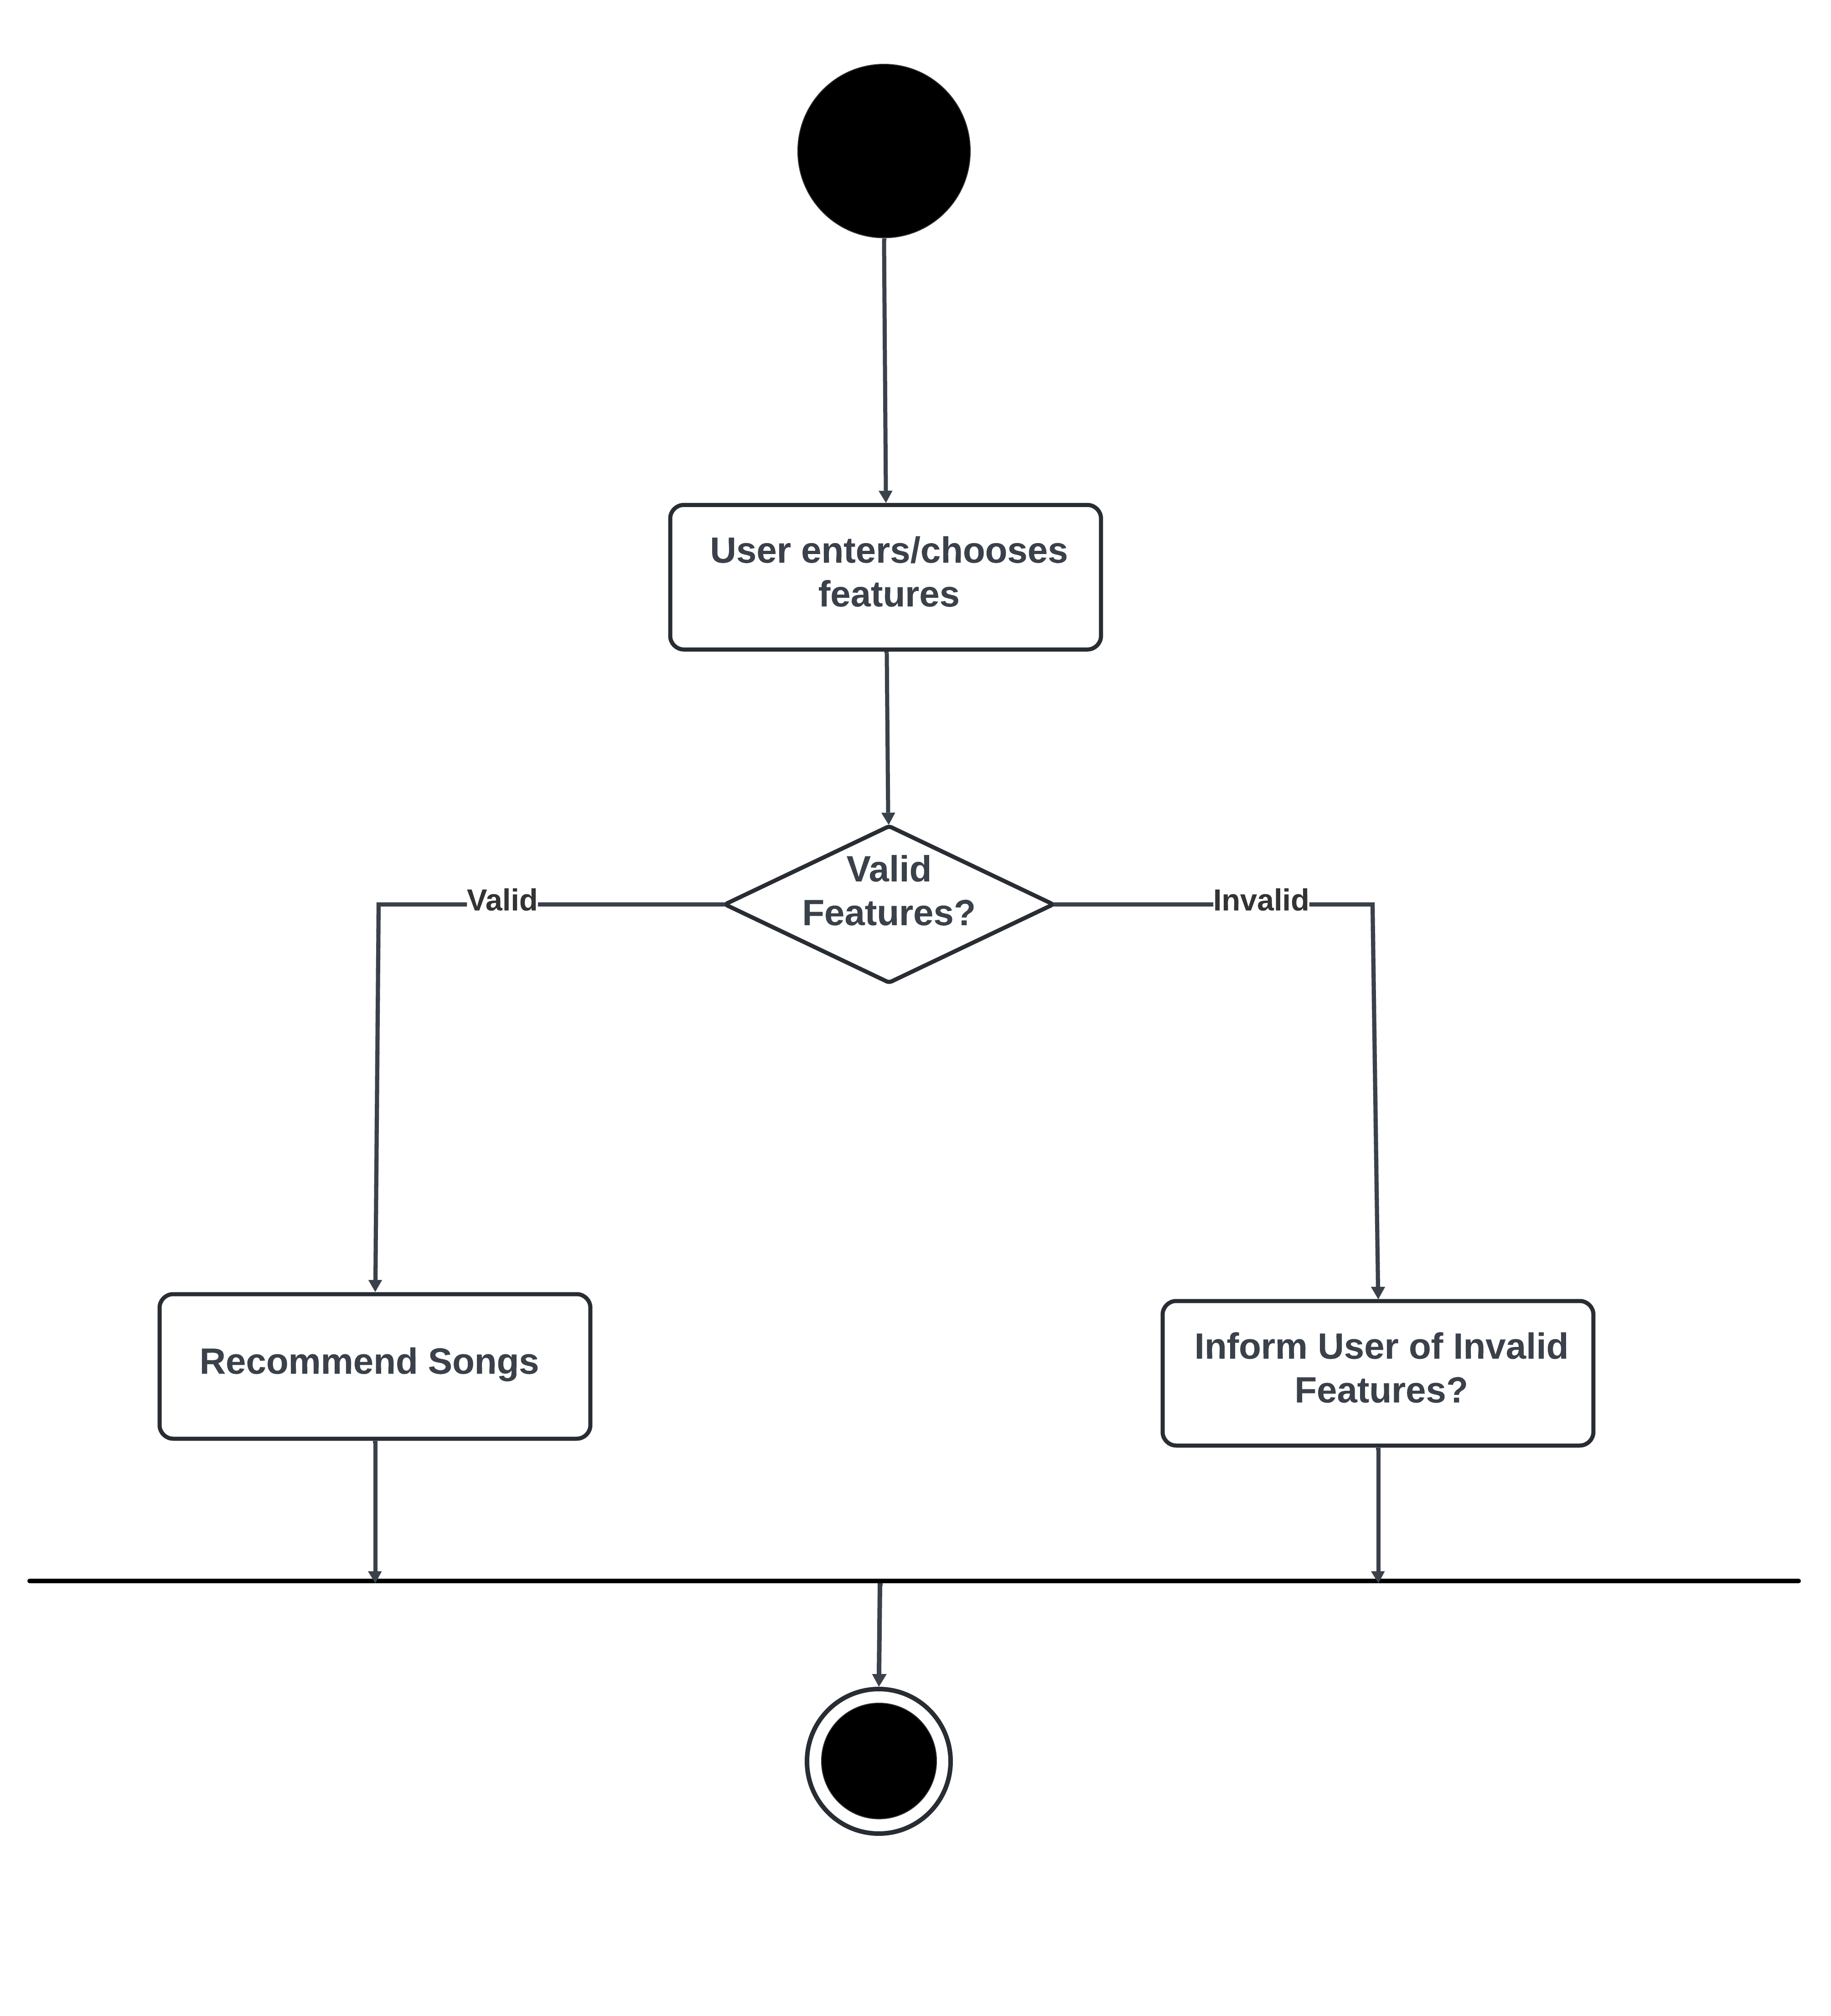
\includegraphics[width=\textwidth]{recommendation_feature.png} \\
\textbf{Outcome:} The user will select or manually enter features they are looking for in a song, and the system will first check to see if the features they selected/entered are valid, and the system will return a collection of reference songs that match those features.

\vspace{1cm}

\noindent \textbf{3. Product Use Case Name:} Music Generation Based on Input \\
\textbf{Trigger:} User inputs reference song(s) and/or song snippet(s), and indicates they want to generate a song \\
\textbf{Preconditions:} User must have GenreGuru open, and the user has provided a valid input(s) \\
\textbf{Interested Stakeholders:} Music producers, Hobbyist Musicians \\
\textbf{Actor/s:} User \\
\textbf{Activity Diagram:} \\
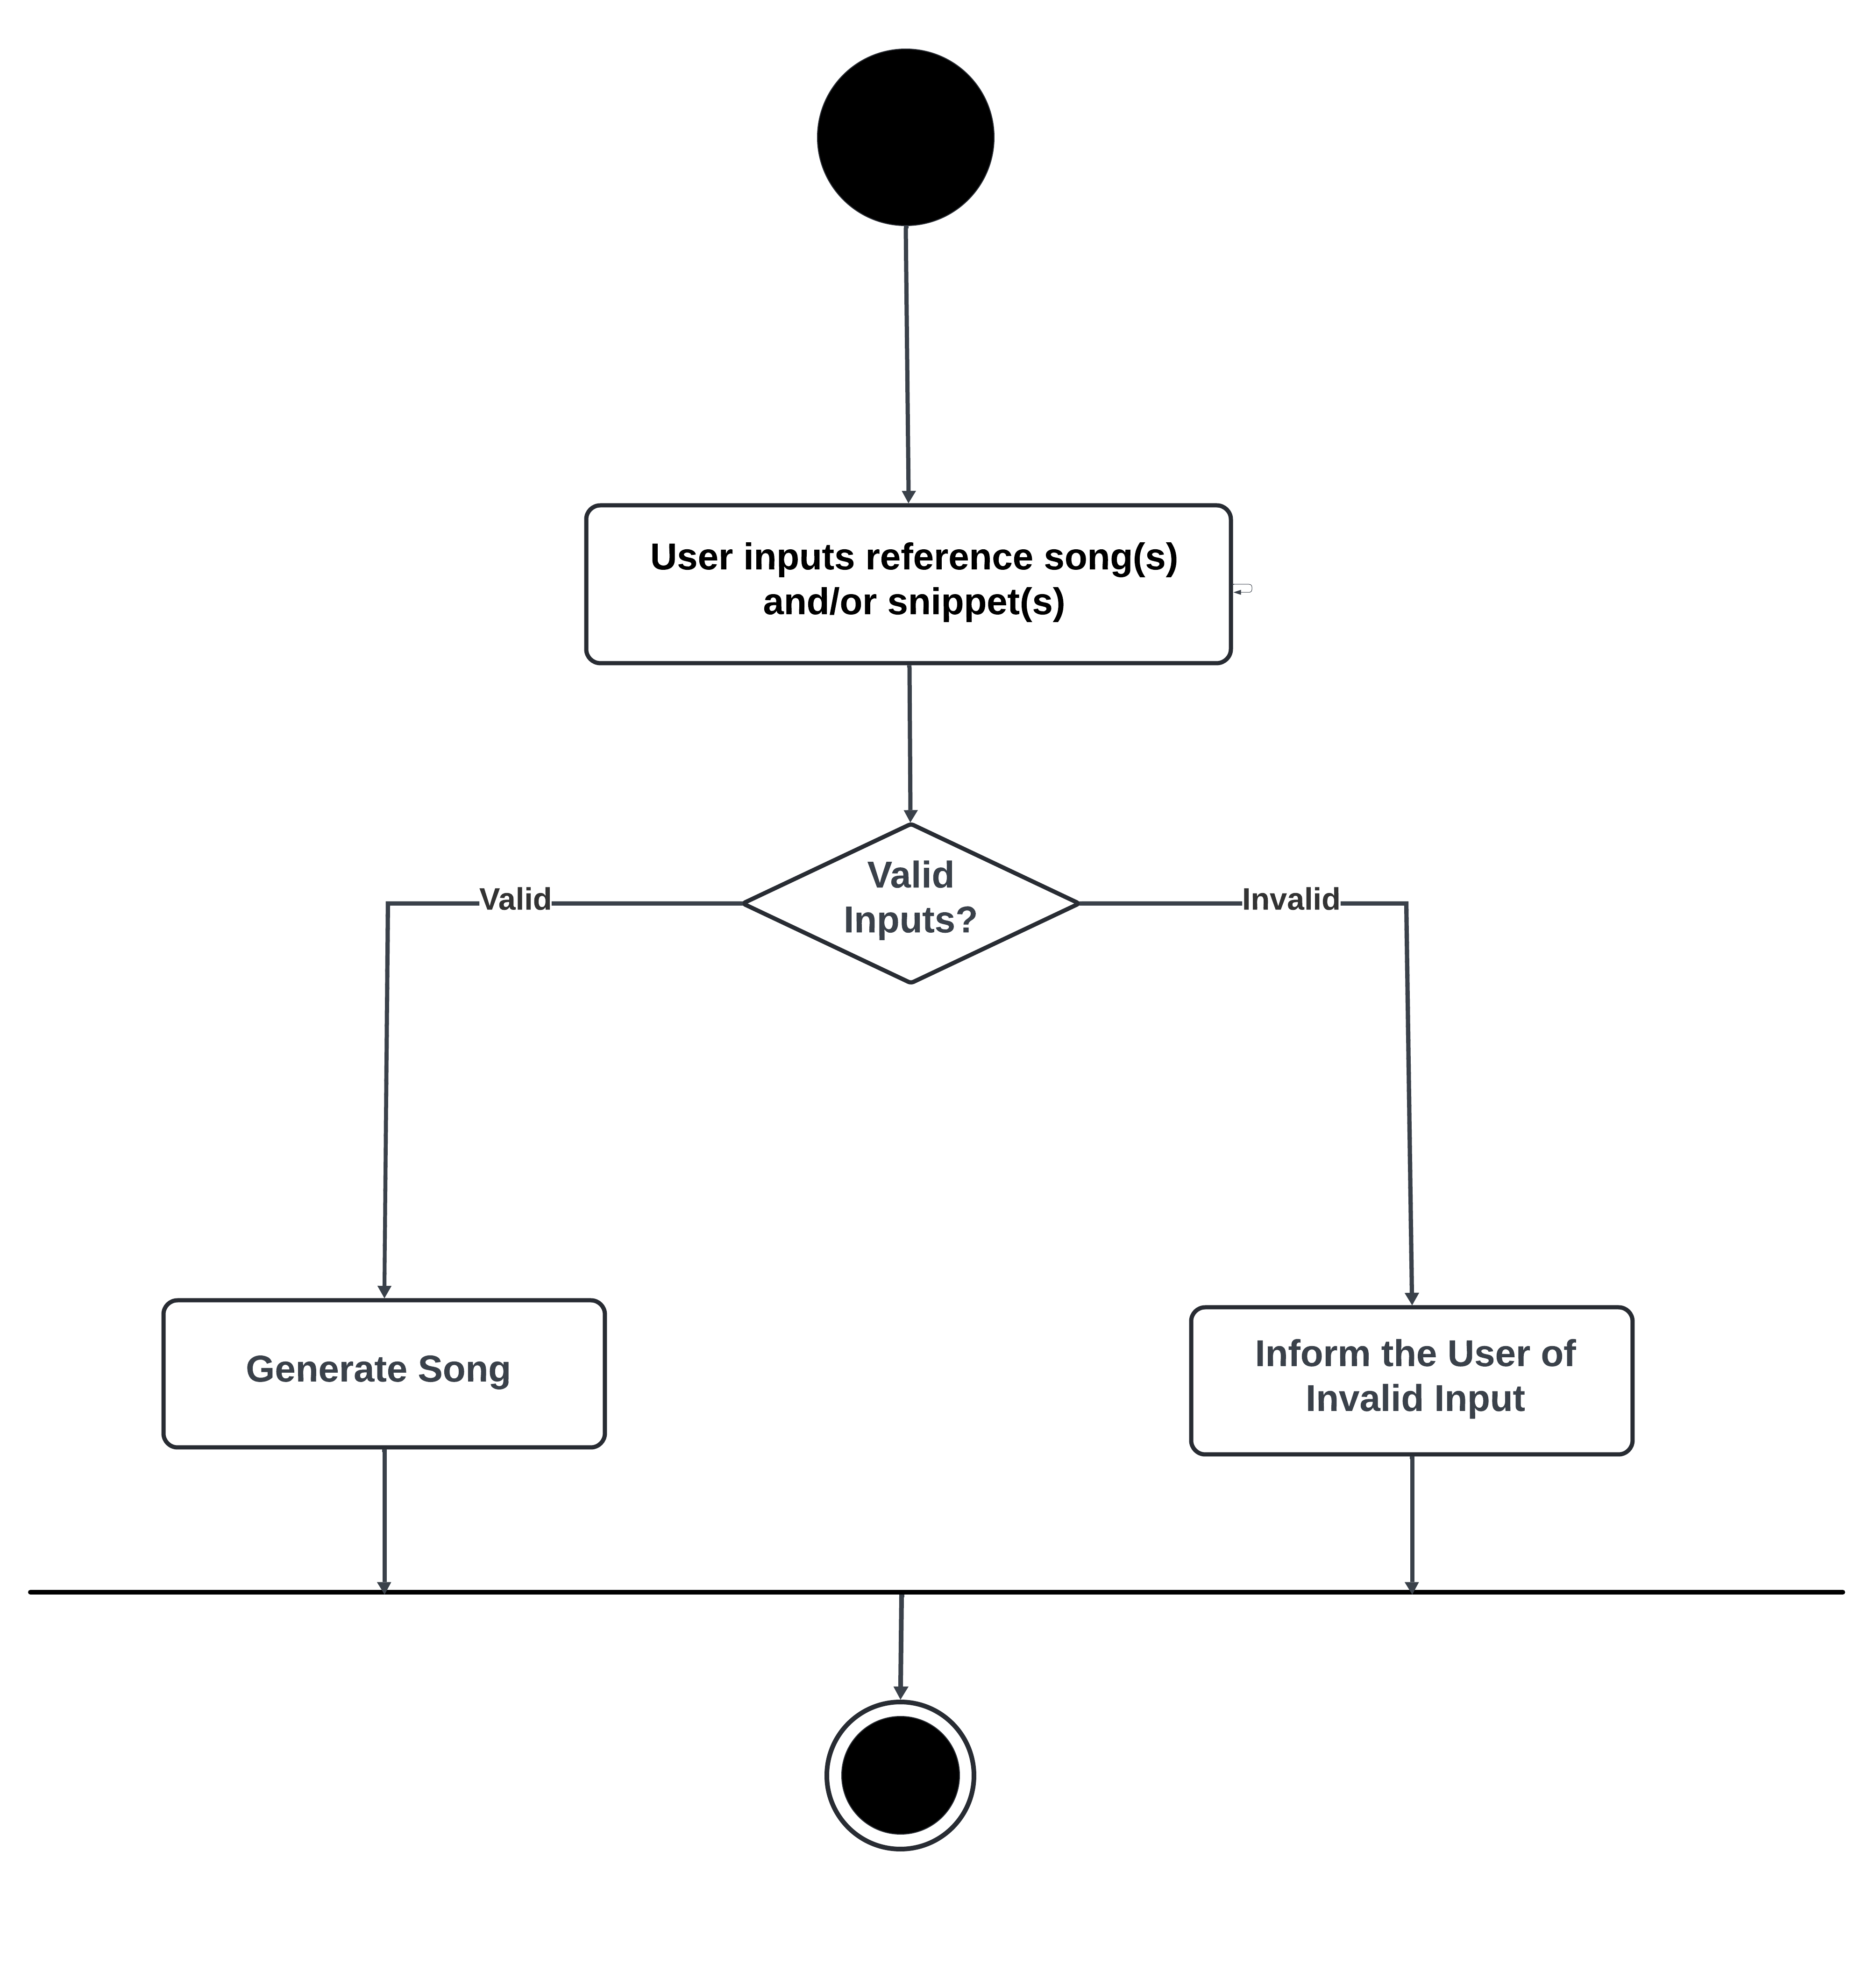
\includegraphics[width=\textwidth]{generate_song.png} \\
\textbf{Outcome:} The user will enter song(s) and/or song snippet(s) and indicate to the system that they want to generate music, the system will check that these inputs are valid (correct format) and then will generate a song and return it to the user.

\vspace{1cm}

\noindent \textbf{4. Product Use Case Name:} Analyze Music \\
\textbf{Trigger:} User inputs a reference song or song snippet and indicates they want to analyze the music \\
\textbf{Preconditions:} User must have GenreGuru open, and the user has provided a valid input \\
\textbf{Interested Stakeholders:} Music Producers, Audio Engineers, Music Educators \\
\textbf{Actor/s:} User \\
\textbf{Activity Diagram:} \\
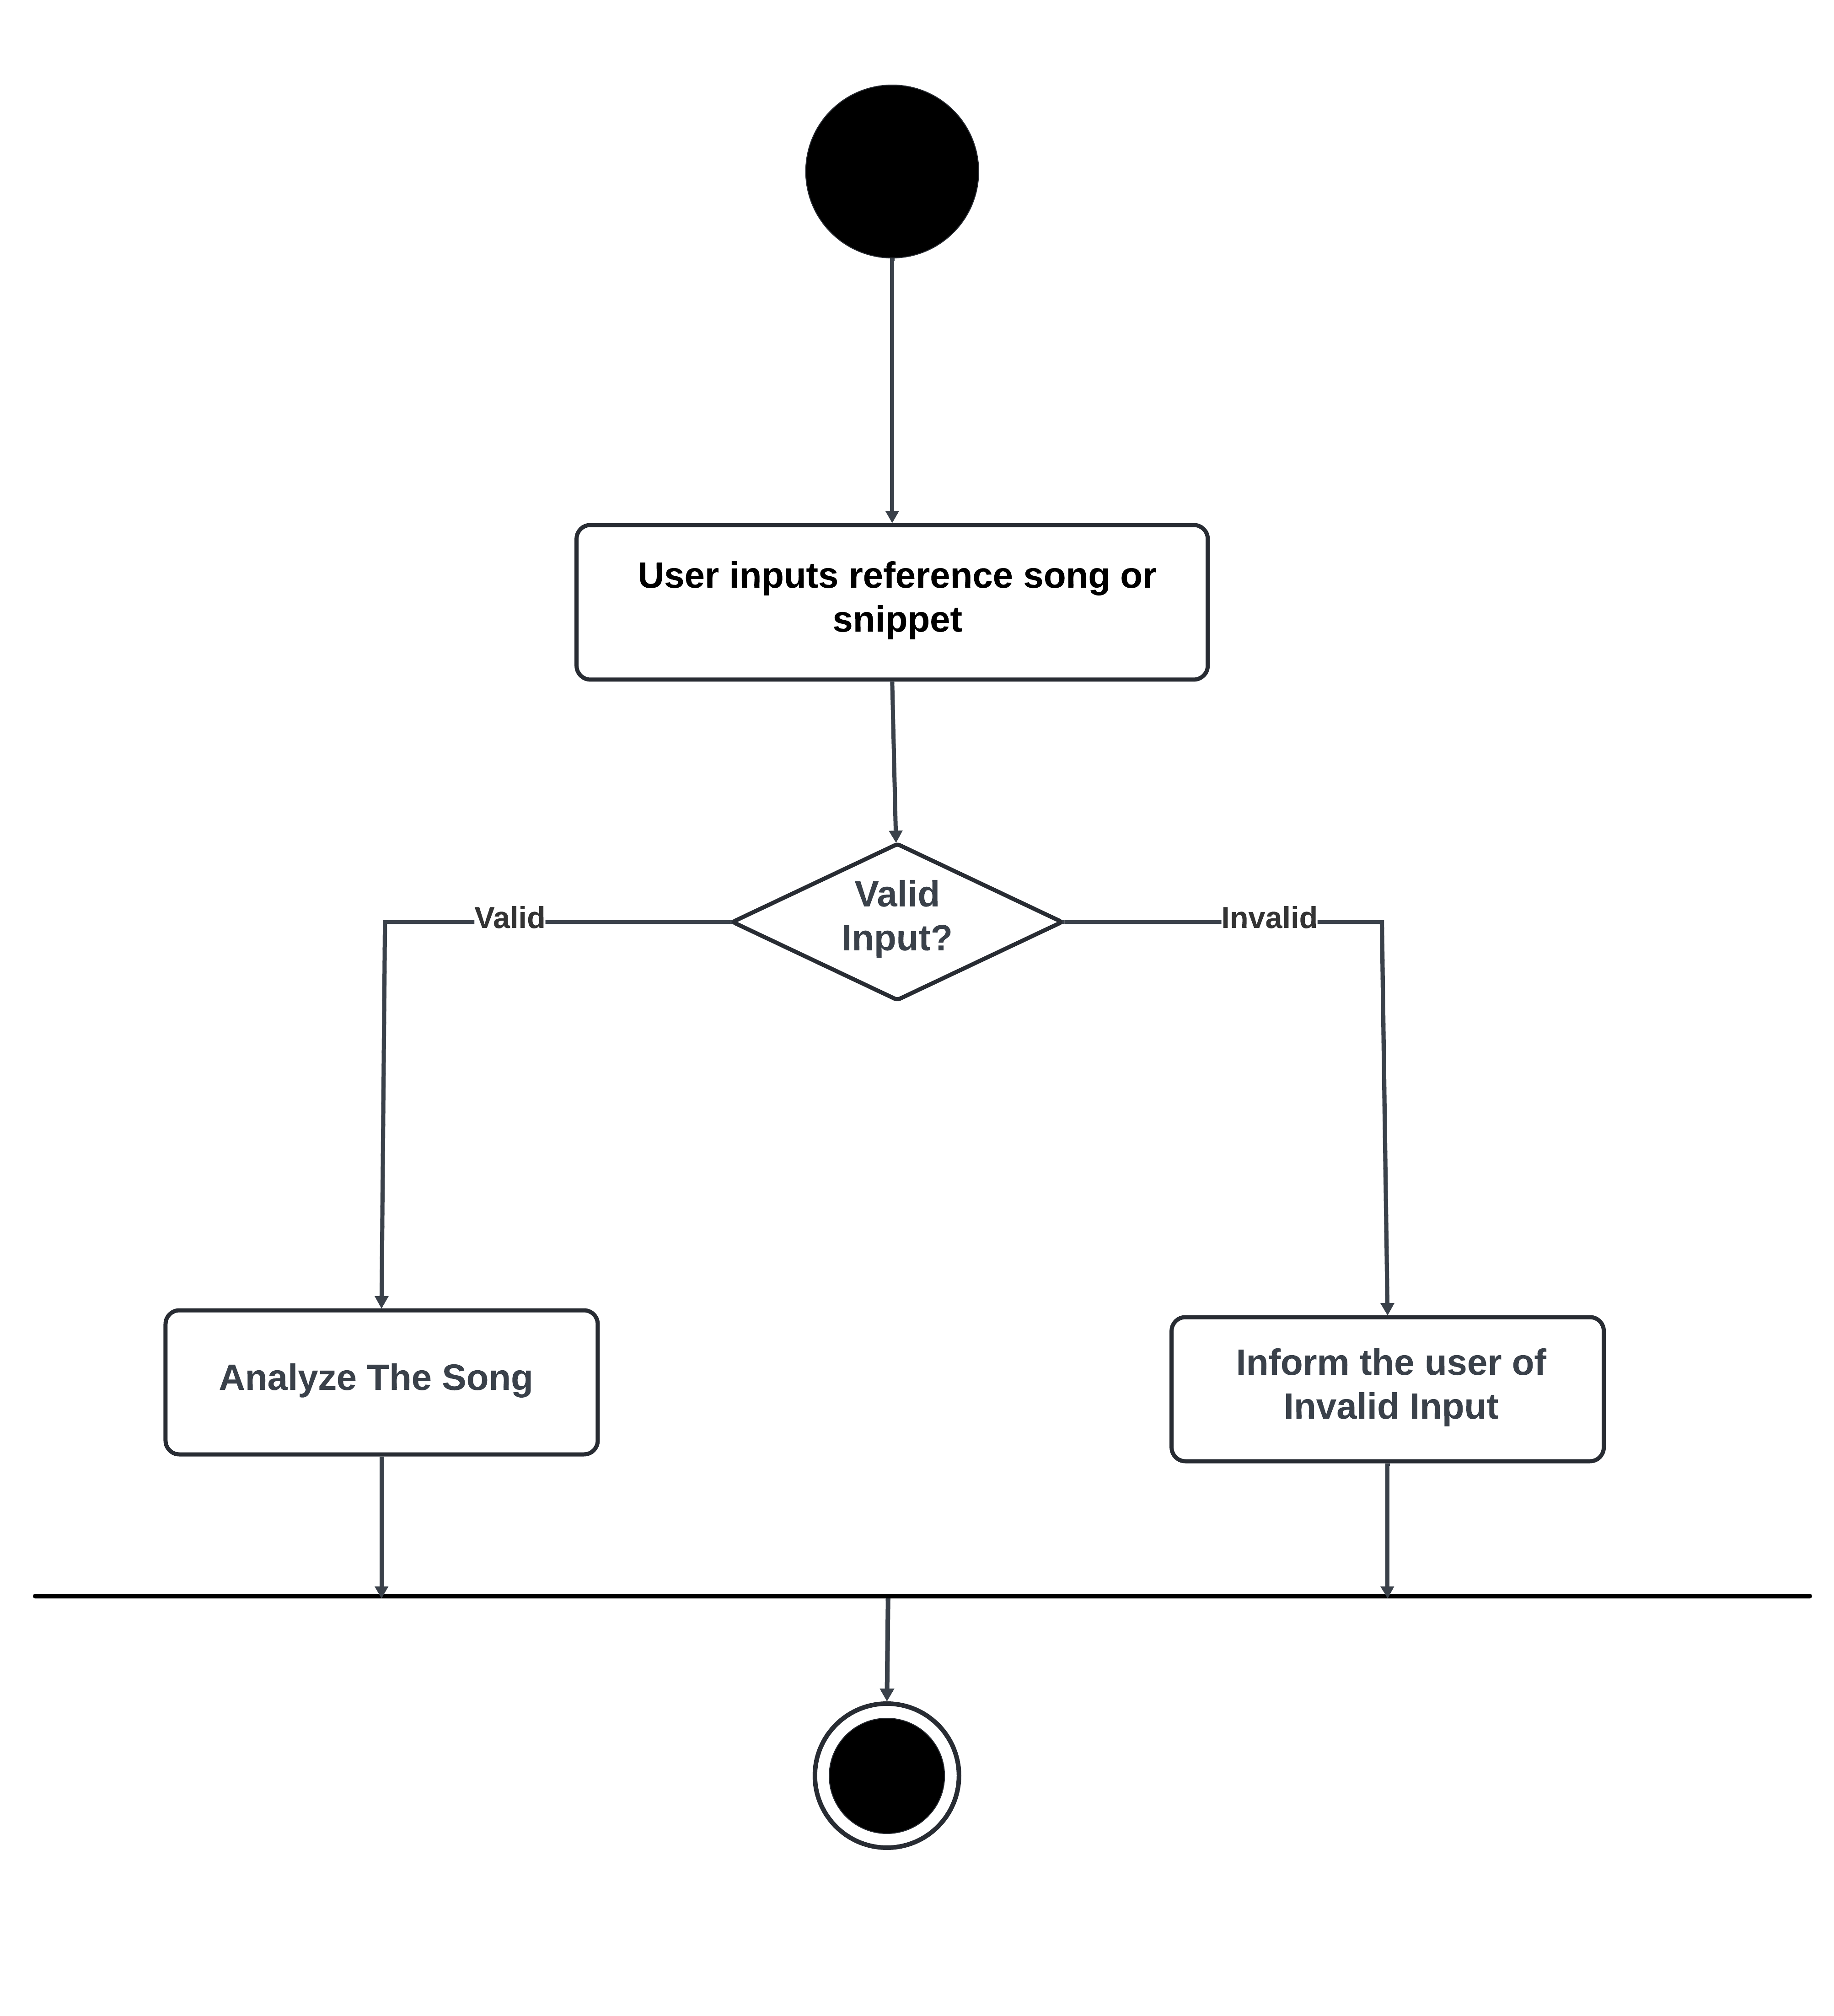
\includegraphics[width=\textwidth]{analyze_song.png} \\
\textbf{Outcome:} The user will input a reference song or song snippet and indicate they want to analyze the song, the system will validate the input and return a set of features and visualizations.

\vspace{1cm}

\noindent \textbf{5. Product Use Case Name:} Song Recommendation Based on Input \\
\textbf{Trigger:} User inputs reference song(s) and/or snippet(s), and indicates they want to search for recommendations \\
\textbf{Preconditions:} User must have GenreGuru open, and the user has provided a valid input(s) \\
\textbf{Interested Stakeholders:} Casual Music Listeners, Hobbyist Musicians \\
\textbf{Actor/s:} User \\
\textbf{Activity Diagram:} \\
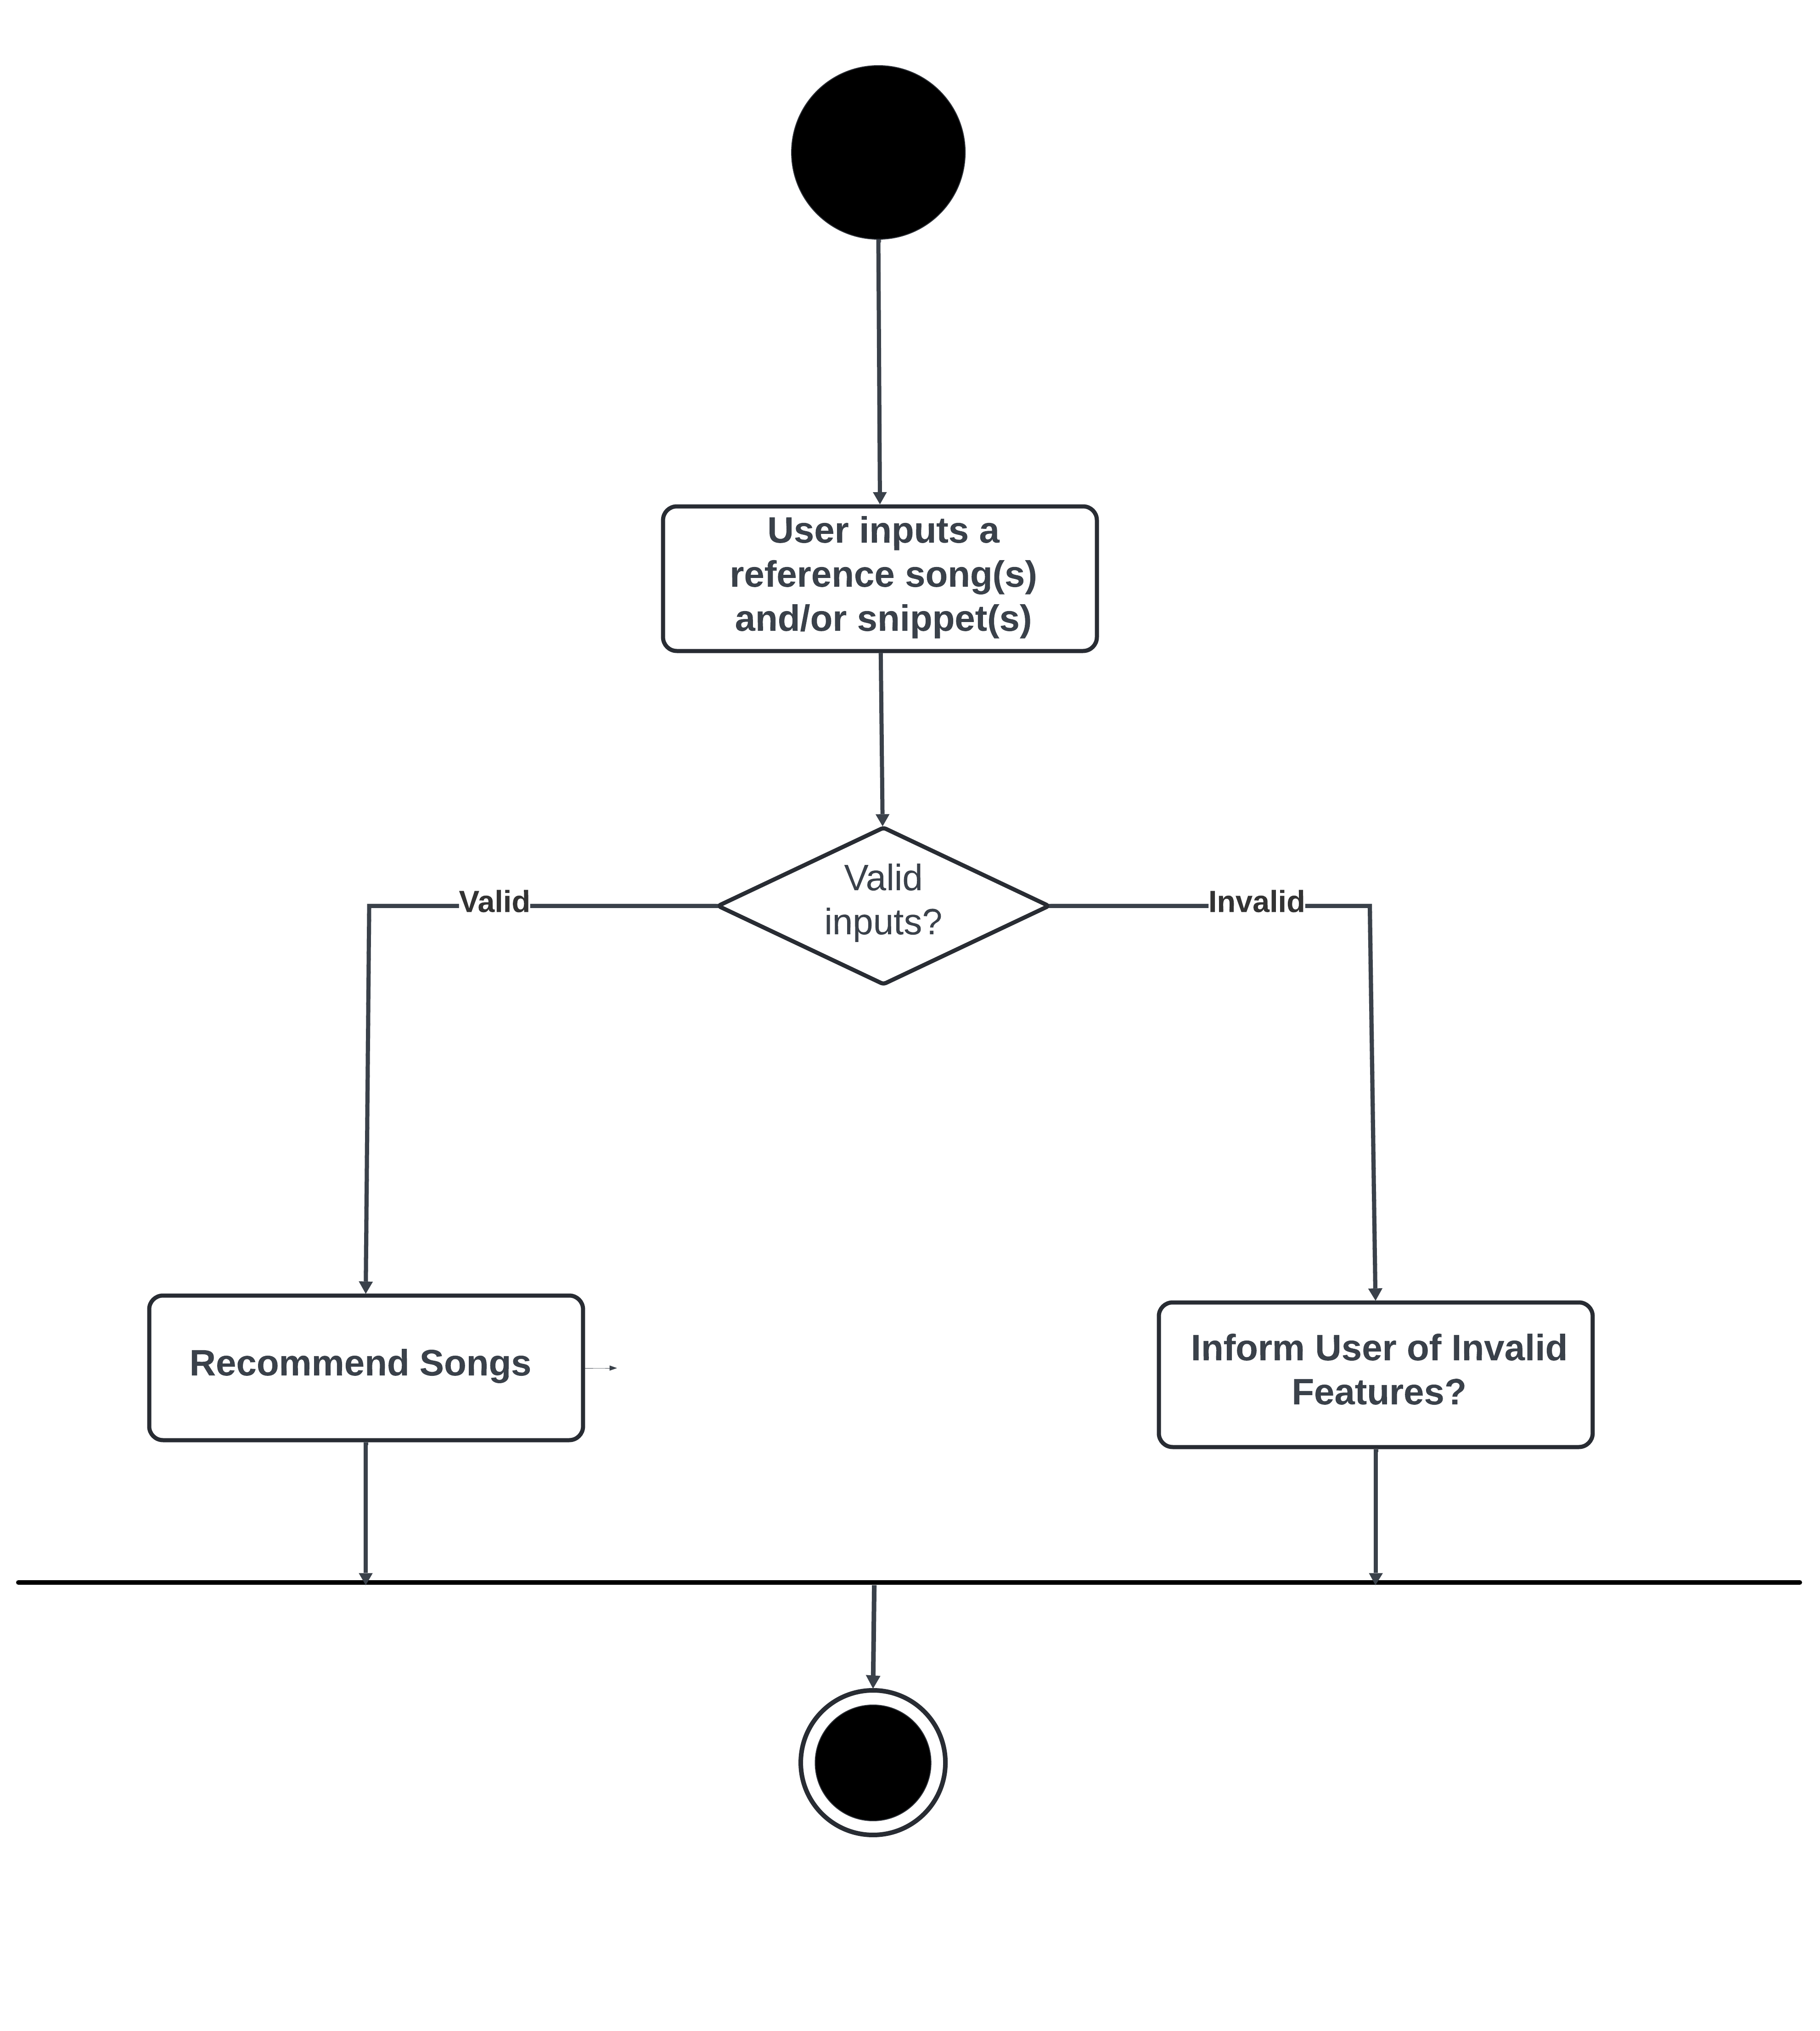
\includegraphics[width=\textwidth]{recommend_song.png} \\
\textbf{Outcome:} The users will input reference song(s) and/or snippet(s), the system will first check to see if the inputs are valid. Then the system will return a collection of reference songs.

\vspace{1cm}

\textbf{6. Product Use Case Name:} Server Interaction for Music Generation \\
\textbf{Trigger:} User submits a reference song and/or snippet and requests music generation \\
\textbf{Preconditions:} User has provided a valid input through, and the server is operational \\
\textbf{Interested Stakeholders:} Music Producers, Hobbyist Musicians \\
\textbf{Actor/s:} Server \\
\textbf{Activity Diagram:} \\
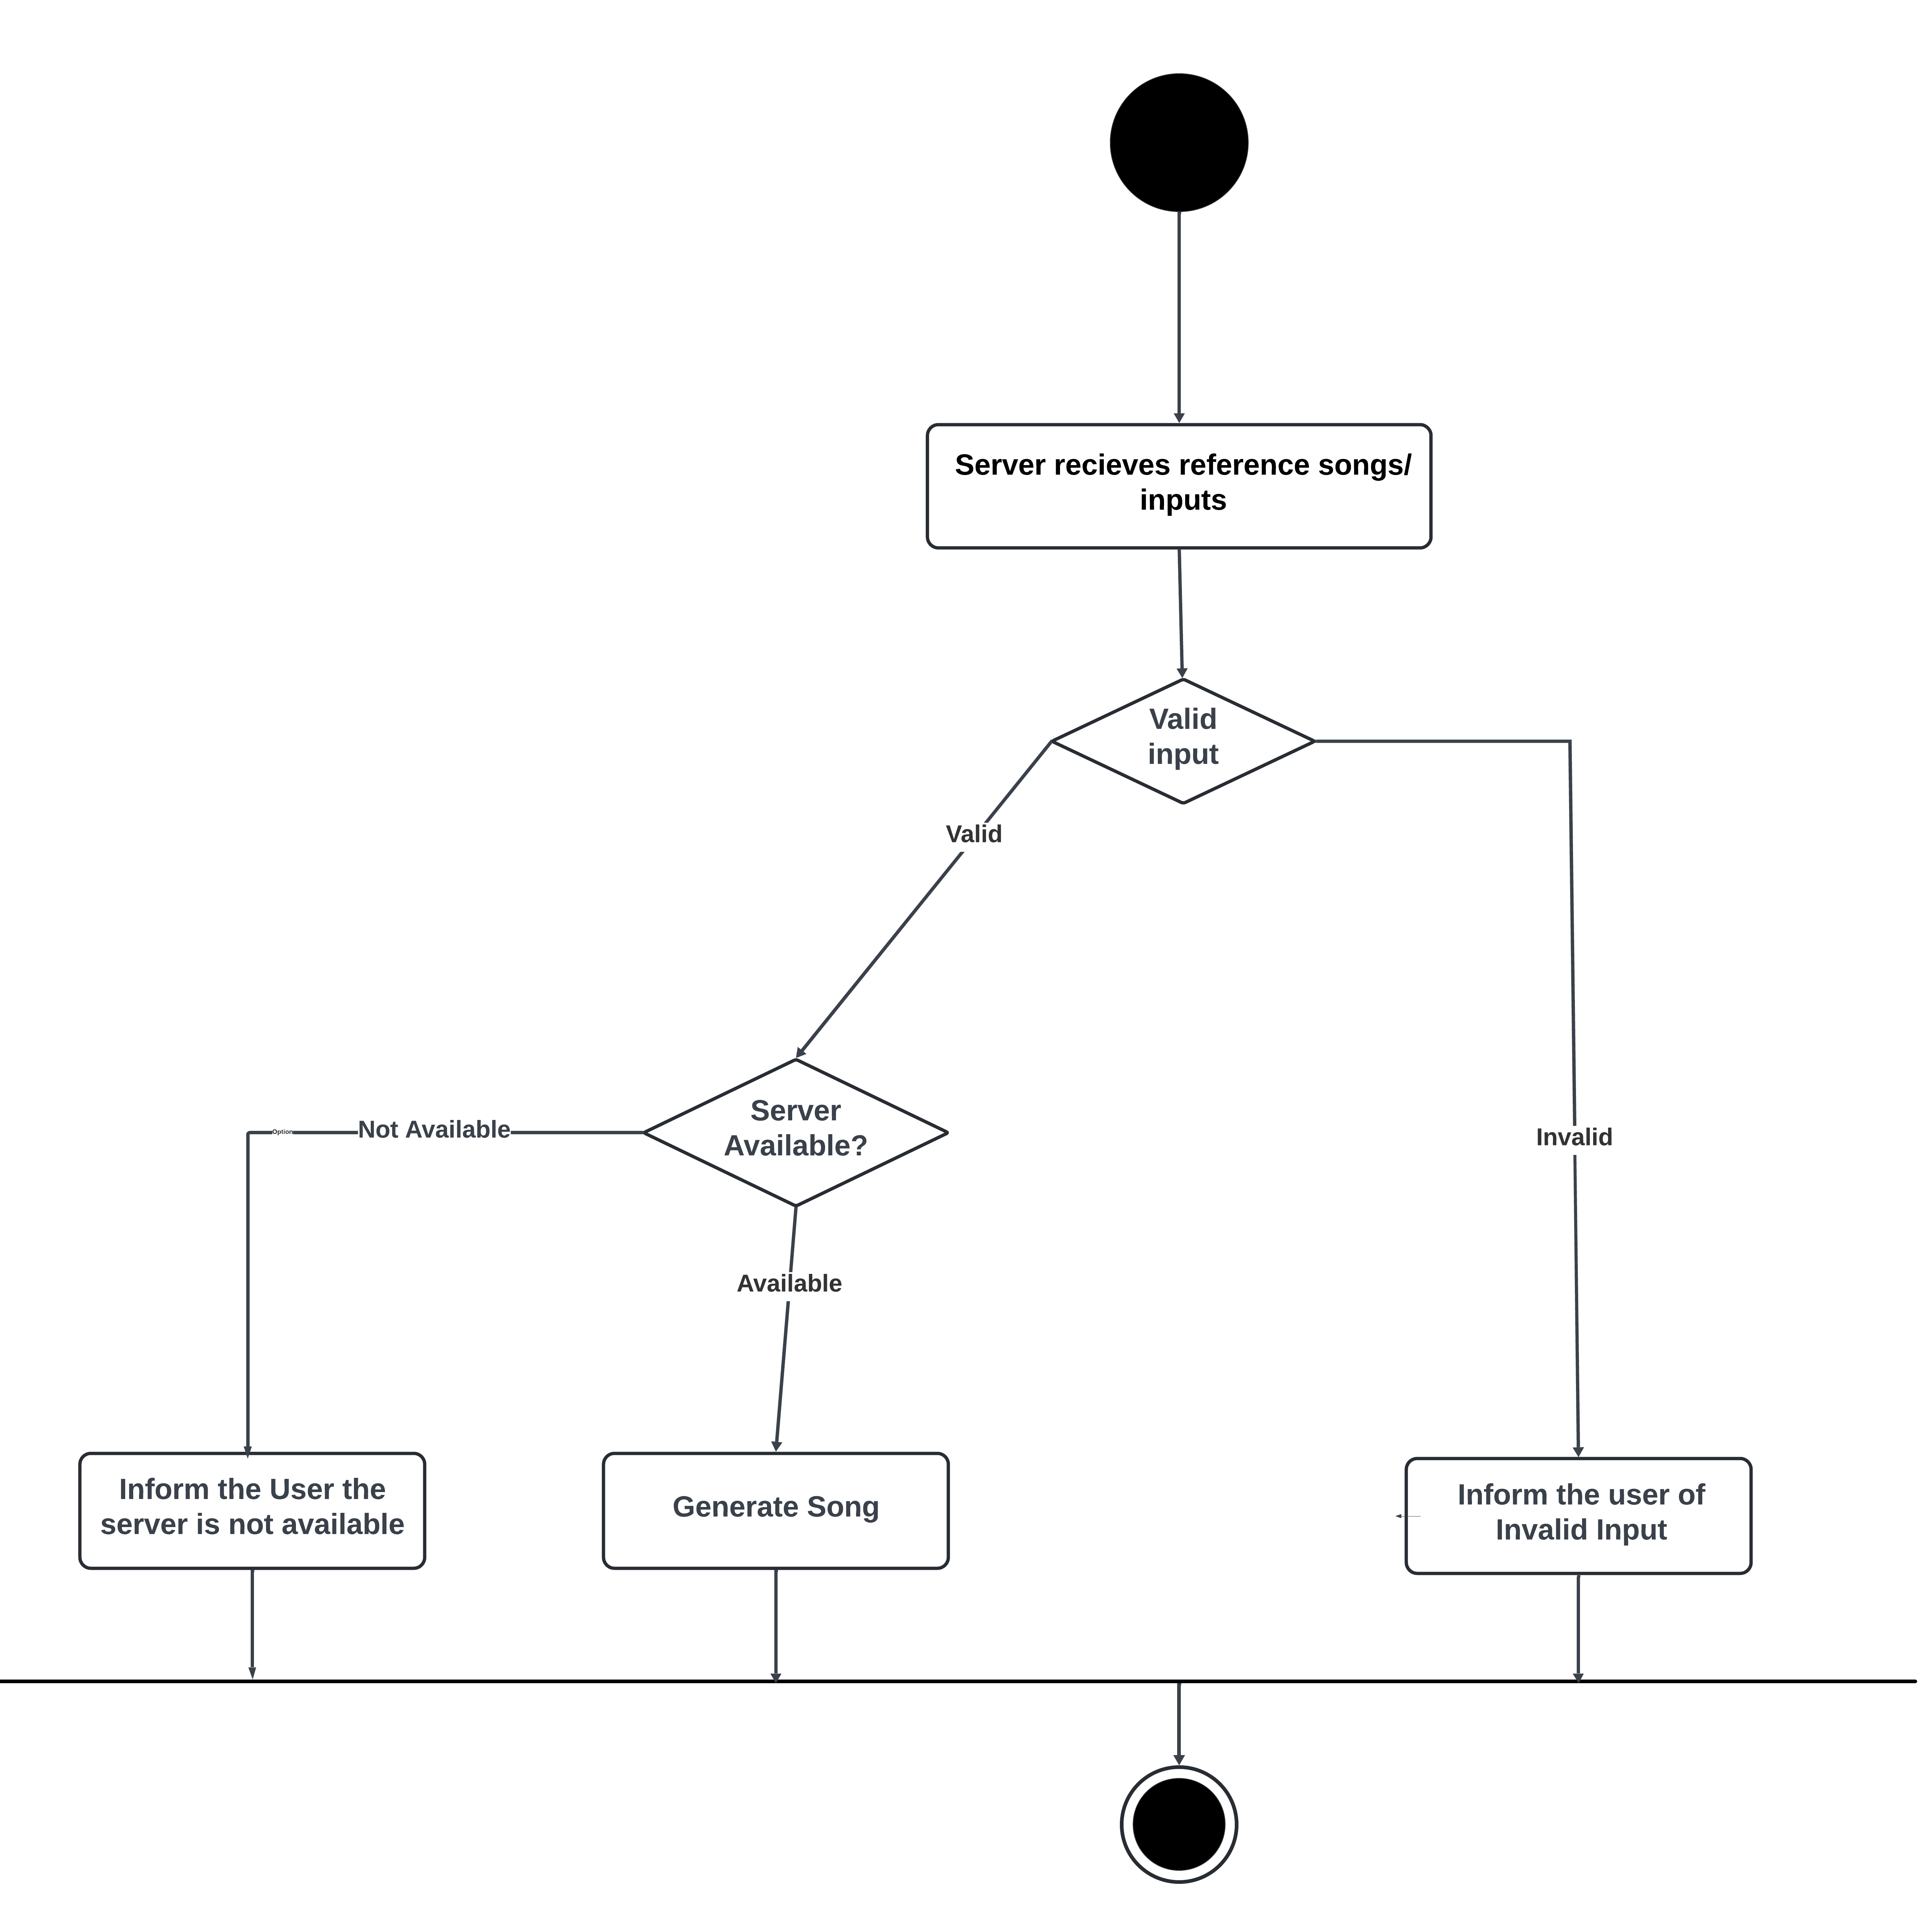
\includegraphics[width=\textwidth]{server_song_gen.png} \\
\textbf{Outcome:} The server processes the input, generates music, and returns the generated song to the user

\vspace{1cm}

\textbf{7. Product Use Case Name:} Server Interaction for Song Recommendation \\
\textbf{Trigger:} User submits desired features or reference songs/snippets and requests song recommendations \\
\textbf{Preconditions:} User has provided valid input, and the server is available \\
\textbf{Interested Stakeholders:} Casual Music Listeners, Hobbyist Musicians \\
\textbf{Actor/s:} Server \\
\textbf{Activity Diagram:} \\
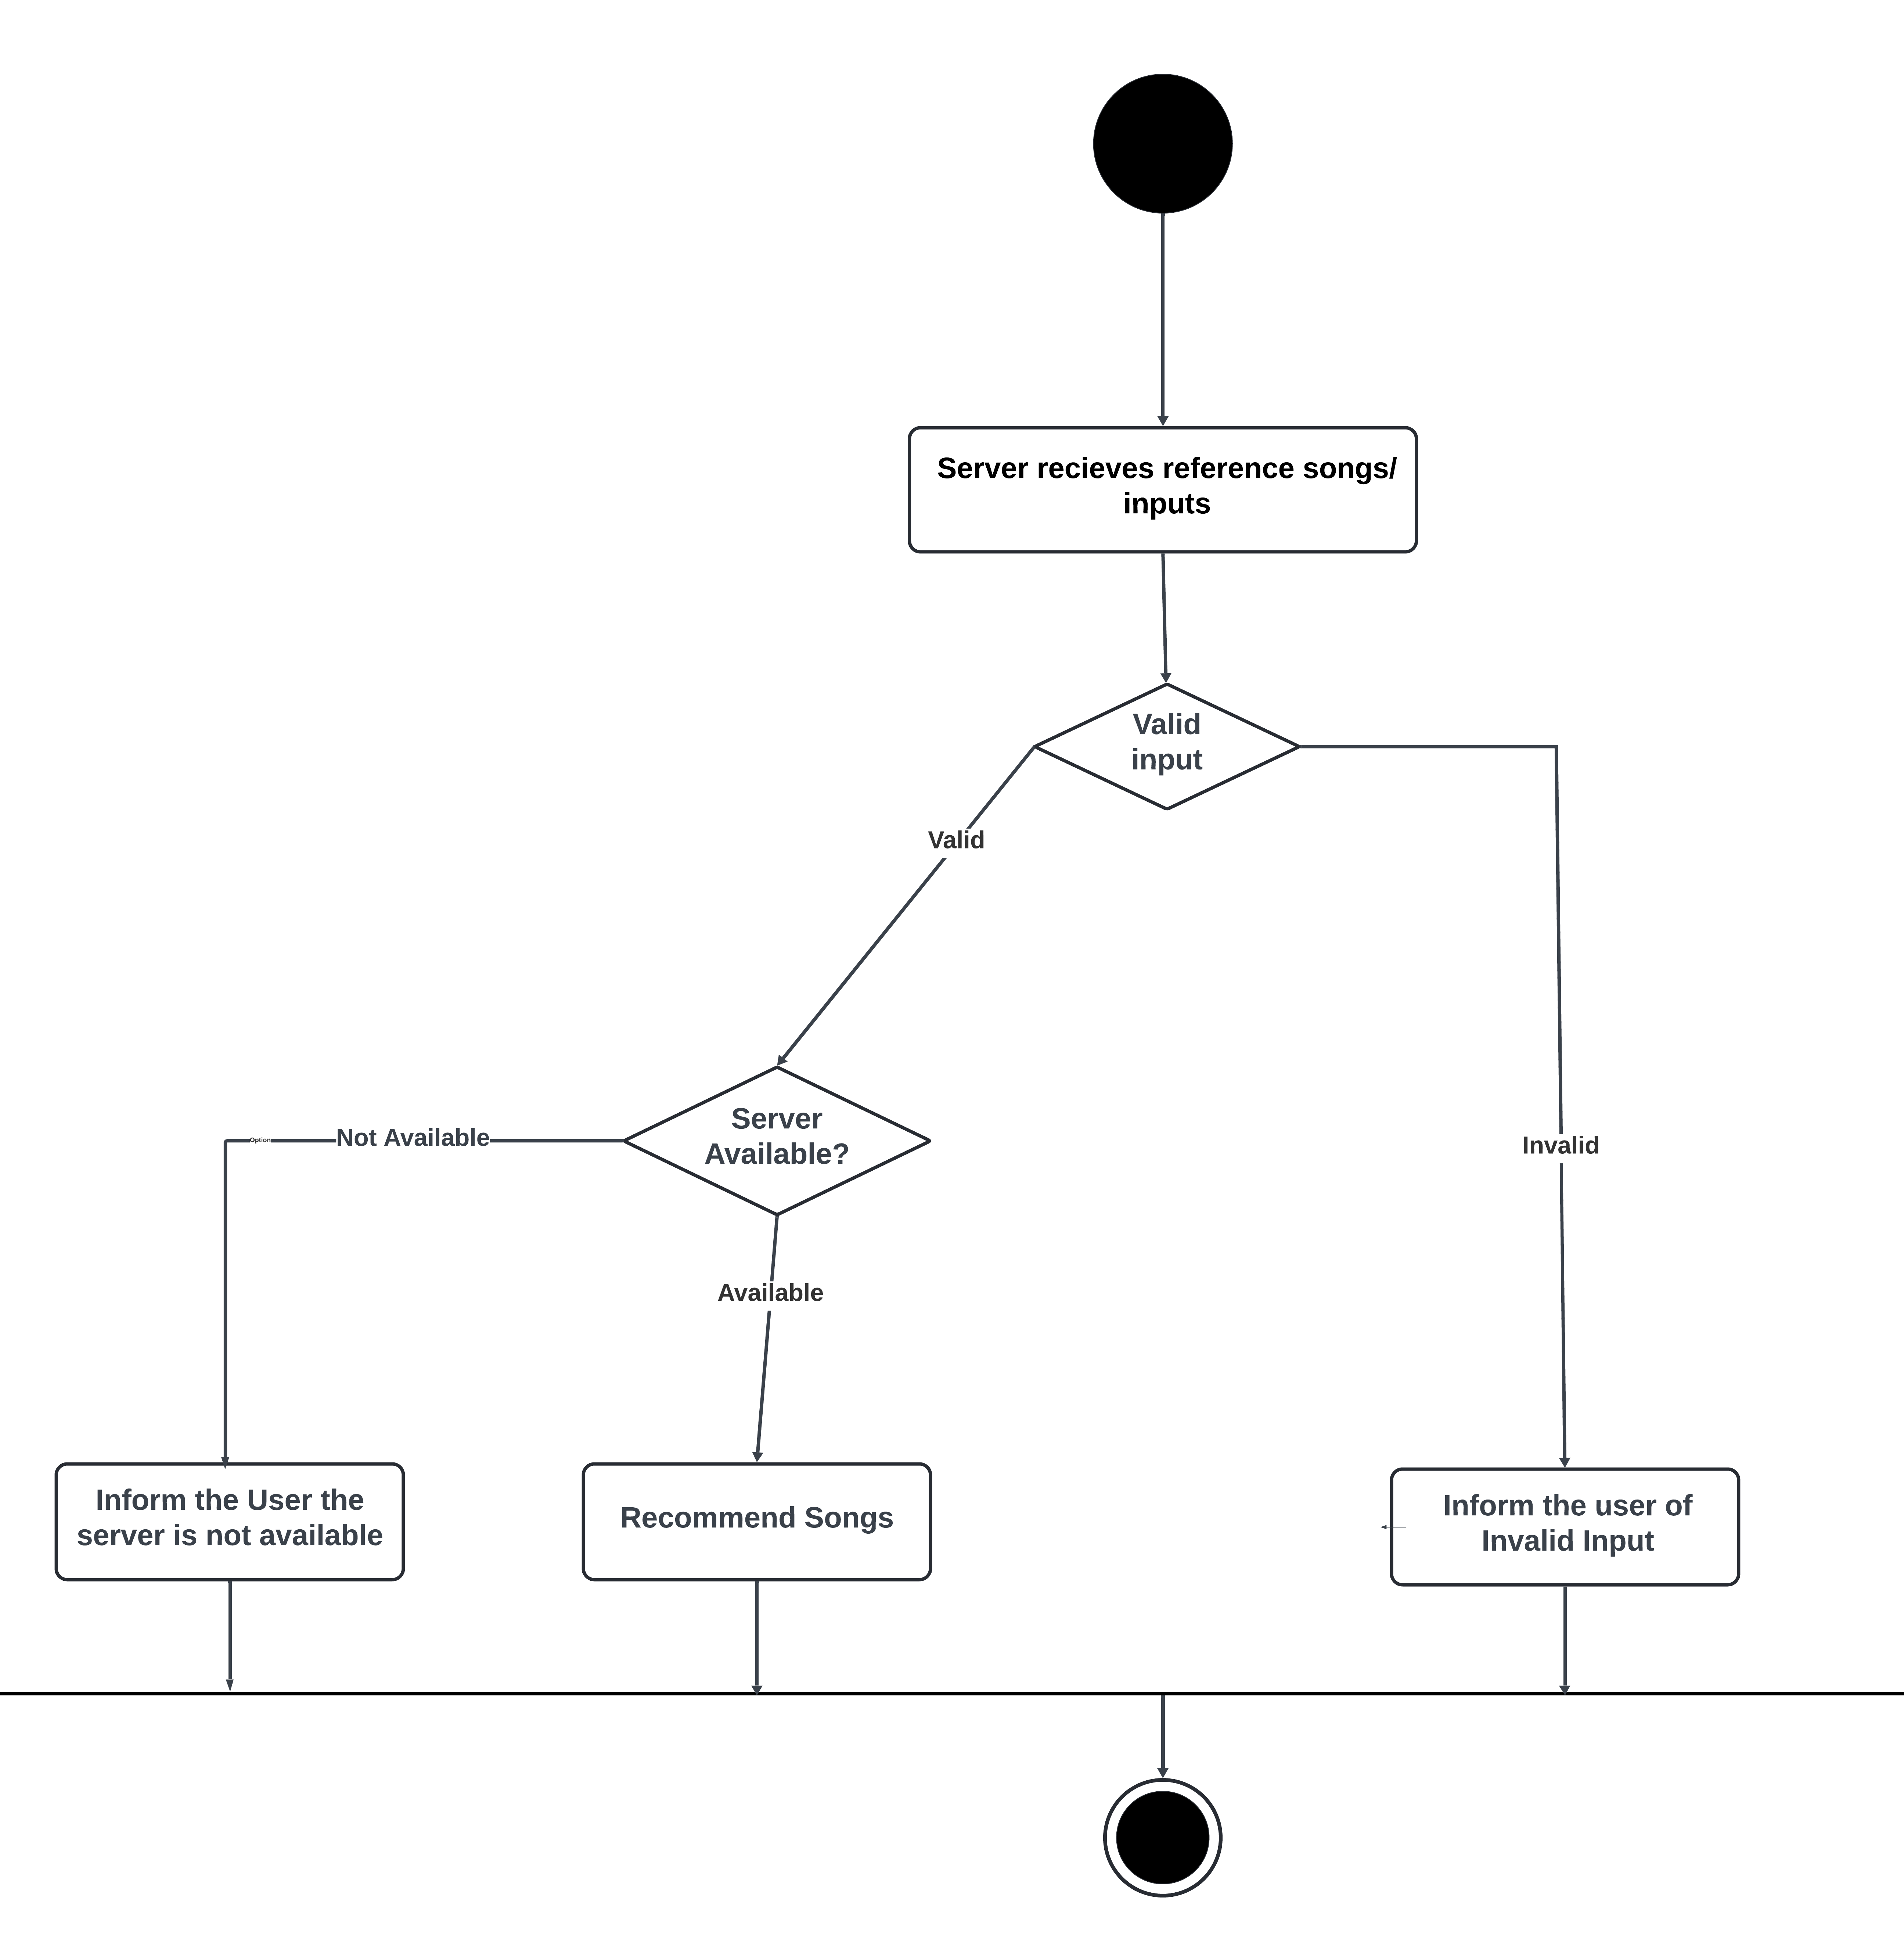
\includegraphics[width=\textwidth]{server_song_rec.png} \\
\textbf{Outcome:} The server processes the input and returns a collection of recommended songs based on the input features or reference songs/snippets.

\vspace{1cm}

\textbf{8. Product Use Case Name:} Server Interaction for Music Analysis \\
\textbf{Trigger:} User submits a reference song or snippet and requests music analysis \\
\textbf{Preconditions:} User has provided a valid input, and the server is ready to analyze \\
\textbf{Interested Stakeholders:} Music Producers, Audio Engineers, Music Educators \\
\textbf{Actor/s:} Server \ \textbf{Activity Diagram:} \\
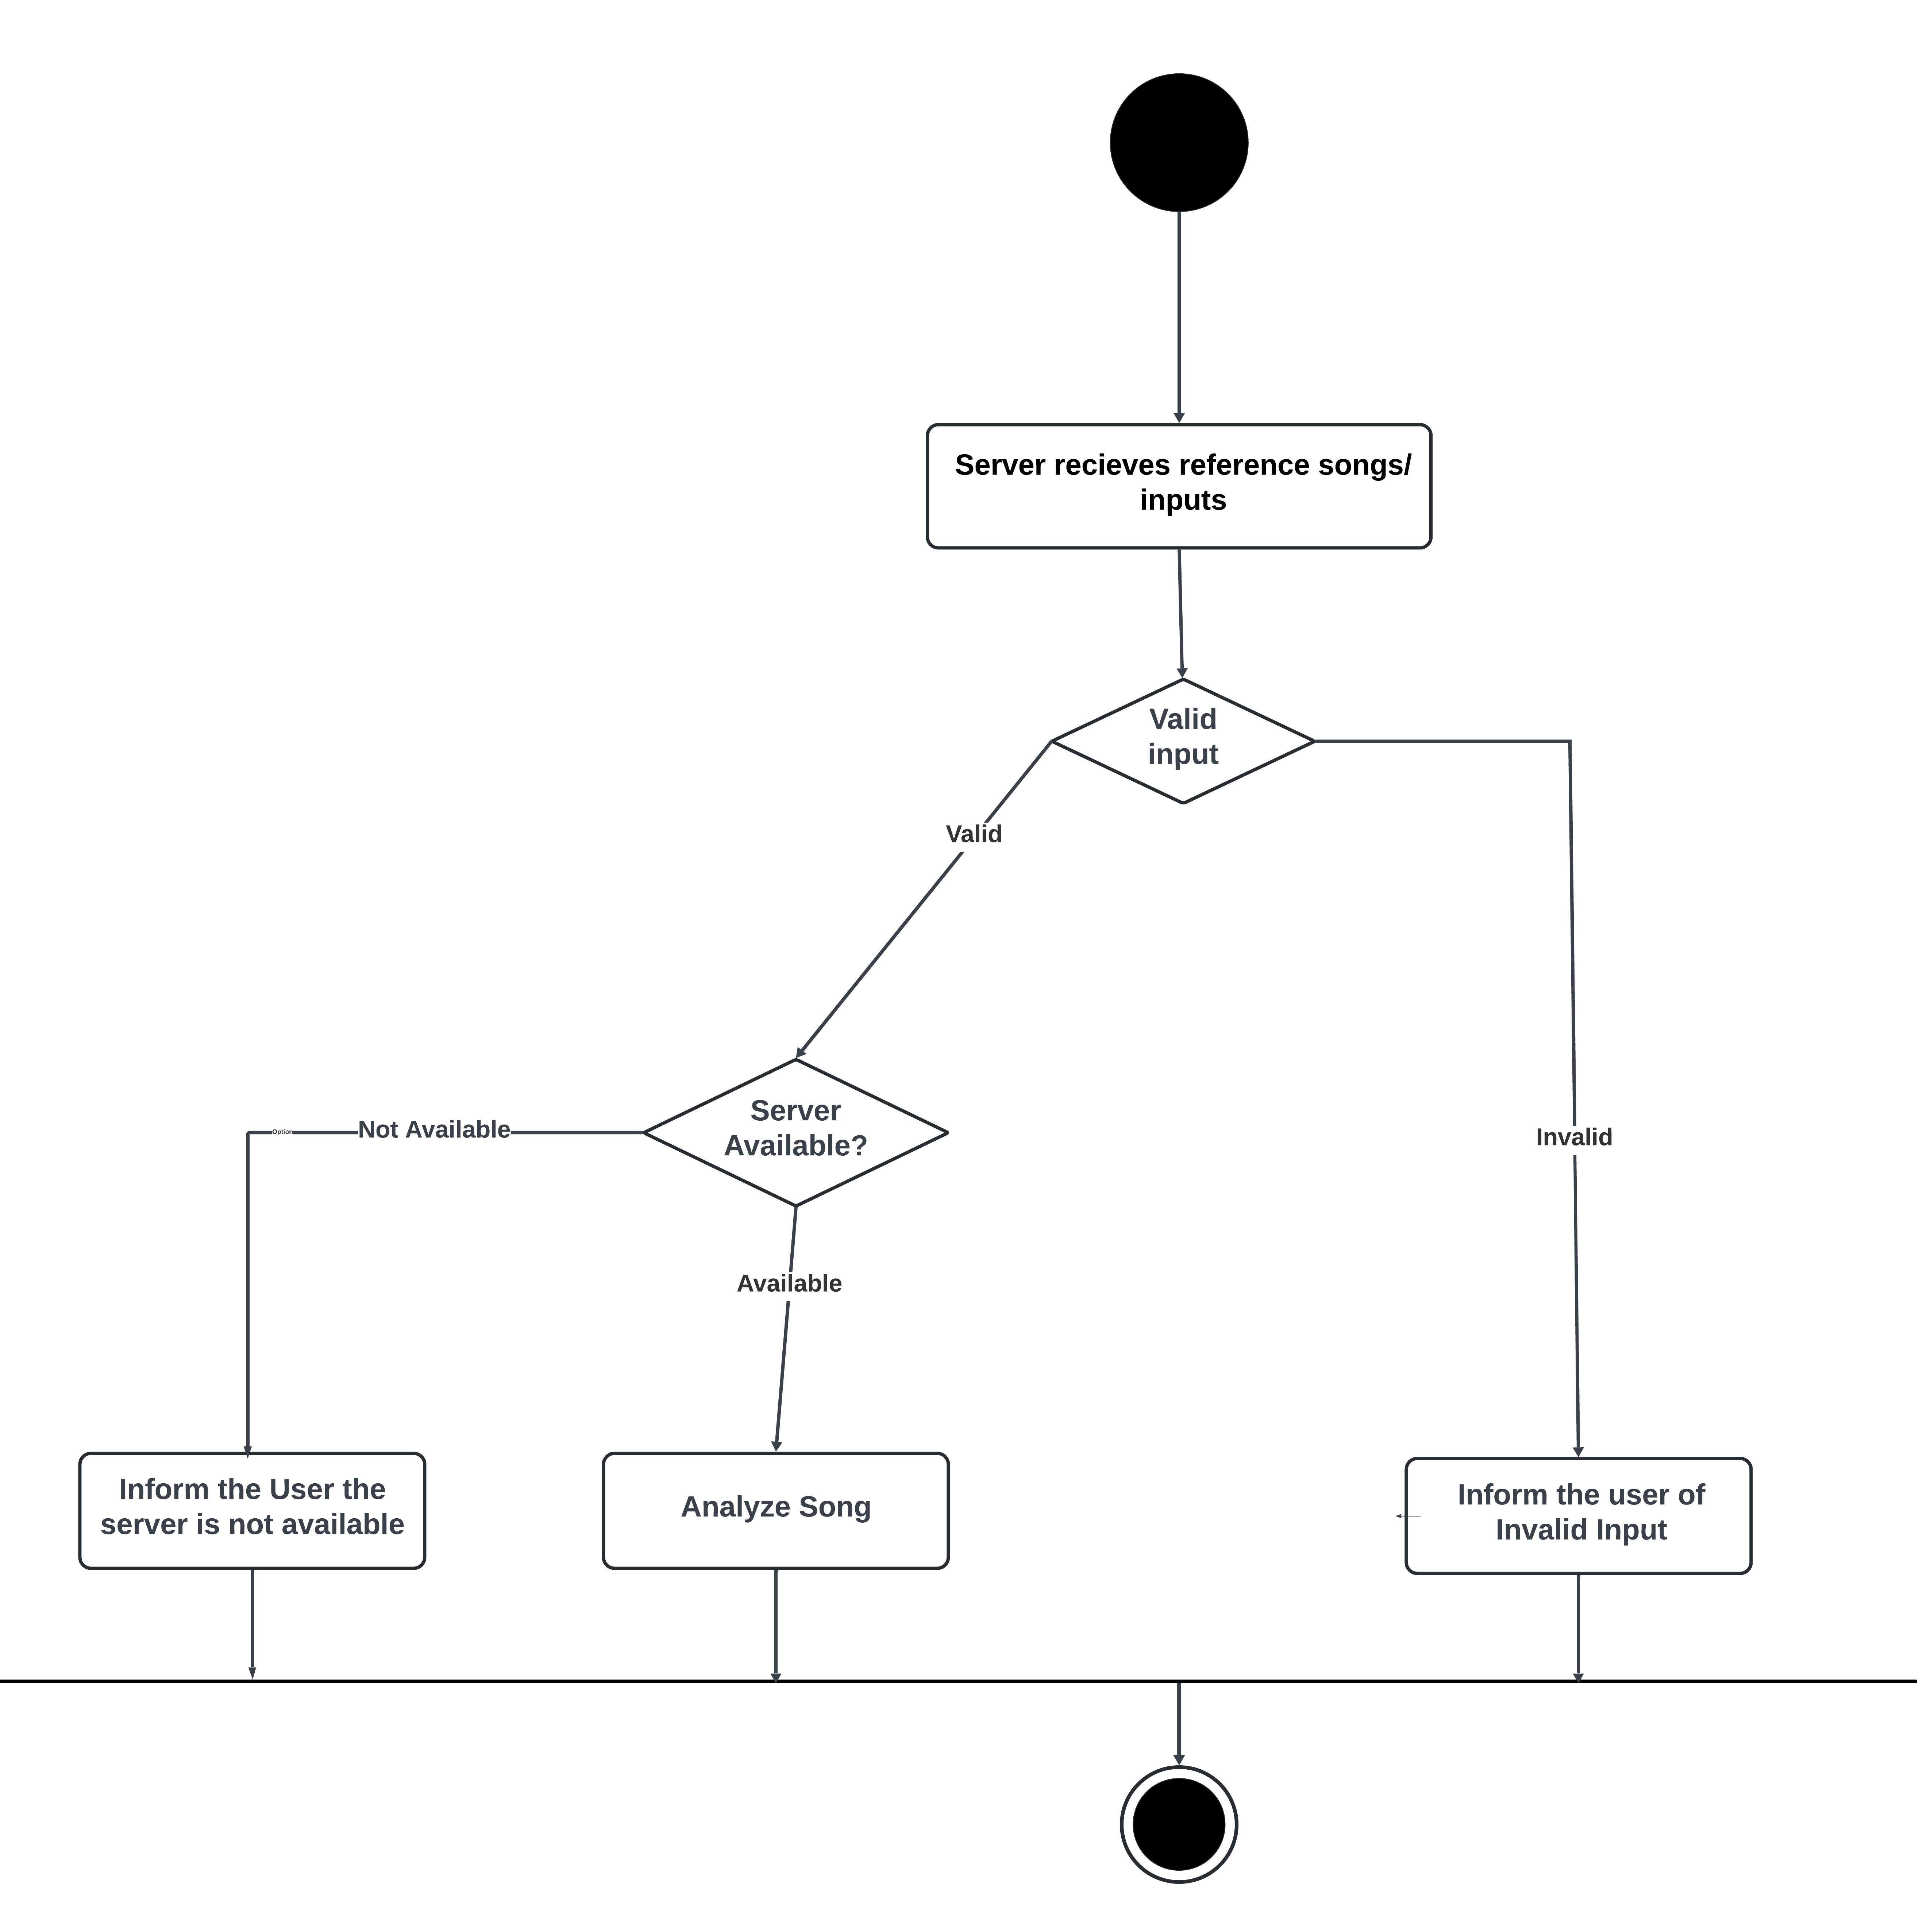
\includegraphics[width=\textwidth]{server_song_analysis.png} \\
\textbf{Outcome:} The server analyzes the song or snippet and returns a collection of features and visualizations to the user.

\section{Functional Requirements}
\subsection{Functional Requirements}
\lips

\section{Look and Feel Requirements}
\subsection{Appearance Requirements}
\lips
\subsection{Style Requirements}
\lips

\section{Usability and Humanity Requirements}
\subsection{Ease of Use Requirements}
\lips
\subsection{Personalization and Internationalization Requirements}
\lips
\subsection{Learning Requirements}
\lips
\subsection{Understandability and Politeness Requirements}
\lips
\subsection{Accessibility Requirements}
\lips

\section{Performance Requirements}
\subsection{Speed and Latency Requirements}
\lips
\subsection{Safety-Critical Requirements}
\lips
\subsection{Precision or Accuracy Requirements}
\lips
\subsection{Robustness or Fault-Tolerance Requirements}
\lips
\subsection{Capacity Requirements}
\lips
\subsection{Scalability or Extensibility Requirements}
\lips
\subsection{Longevity Requirements}
\lips

\section{Operational and Environmental Requirements}
\subsection{Expected Physical Environment}
\lips
\subsection{Wider Environment Requirements}
\lips
\subsection{Requirements for Interfacing with Adjacent Systems}
\lips
\subsection{Productization Requirements}
\lips
\subsection{Release Requirements}
\lips

\section{Maintainability and Support Requirements}
\subsection{Maintenance Requirements}
\lips
\subsection{Supportability Requirements}
\lips
\subsection{Adaptability Requirements}
\lips

\section{Security Requirements}
\subsection{Access Requirements}
\lips
\subsection{Integrity Requirements}
\lips
\subsection{Privacy Requirements}
\lips
\subsection{Audit Requirements}
\lips
\subsection{Immunity Requirements}
\lips

\section{Cultural Requirements}
\subsection{Cultural Requirements}
\lips

\section{Compliance Requirements}
\subsection{Legal Requirements}
\lips
\subsection{Standards Compliance Requirements}
\lips

\section{Open Issues}
\lips

\section{Off-the-Shelf Solutions}
\subsection{Ready-Made Products}
\lips
\subsection{Reusable Components}
\lips
\subsection{Products That Can Be Copied}
\lips

\section{New Problems}
\subsection{Effects on the Current Environment}
\lips
\subsection{Effects on the Installed Systems}
\lips
\subsection{Potential User Problems}
\lips
\subsection{Limitations in the Anticipated Implementation Environment That May
Inhibit the New Product}
\lips
\subsection{Follow-Up Problems}
\lips

\section{Tasks}
\subsection{Project Planning}
\lips
\subsection{Planning of the Development Phases}
\lips

\section{Migration to the New Product}
\subsection{Requirements for Migration to the New Product}
\lips
\subsection{Data That Has to be Modified or Translated for the New System}
\lips

\section{Costs}
\lips
\section{User Documentation and Training}
\subsection{User Documentation Requirements}
\lips
\subsection{Training Requirements}
\lips

\section{Waiting Room}
\lips

\section{Ideas for Solution}
\lips

\newpage{}
\section*{Appendix --- Reflection}

The information in this section will be used to evaluate the team members on the
graduate attribute of Lifelong Learning.  Please answer the following questions:

\begin{enumerate}
  \item What knowledge and skills will the team collectively need to acquire to
  successfully complete this capstone project?  Examples of possible knowledge
  to acquire include domain specific knowledge from the domain of your
  application, or software engineering knowledge, mechatronics knowledge or
  computer science knowledge.  Skills may be related to technology, or writing,
  or presentation, or team management, etc.  You should look to identify at
  least one item for each team member.
  \item For each of the knowledge areas and skills identified in the previous
  question, what are at least two approaches to acquiring the knowledge or
  mastering the skill?  Of the identified approaches, which will each team
  member pursue, and why did they make this choice?
\end{enumerate}

\end{document}